\documentclass{article}
\usepackage{amscd,amssymb,amsmath,latexsym,graphicx,epsfig,color,url,todonotes,geometry}
\geometry{margin=1.3in}
\usepackage{graphicx} % Required for inserting images

\newcommand{\red}{\textcolor{red}}
\newcommand{\blue}{\textcolor{blue}}
\newcommand{\black}{\textcolor{black}}
\newcommand{\green}{\textcolor{green}}

\newcommand{\Res}{\operatorname{Res}}
\title{Superfluids}
\author{Eloi Estèvez \and Eki González \and Joan Pascual \and Timothy David Skipper}
\date{\today}

\begin{document}

\maketitle
\begin{abstract}
\todo{Write abstract}
\end{abstract}

\tableofcontents
\newpage

\section{Bose-Einstein condensates}

Could quantum physics help us explain the strange behaviour of helium II?  In 1938, Fritz London proposed that Bose-Einstein condensates could be a mechanism for superfluidity.  This makes sense since helium 4 atoms are bosons: they are made up of an even number of fermions (2 protons, 2 neutrons and 2 electrons).  In 1924 Satyendra Nath Bose was the first to study these types of particles and their statistical behaviour.  Among other things, he considered the possibility of cooling down such a system to very low temperatures, and sent his work to Einstein for translation.  Einstein recognised the value of his efforts and agreed to translate the paper to German, and further made his own contributions.
Before even talking about superfluids, we...

\subsection{Basics}

A Bose-Einstein condensate is a many-particle system which, due to certain
conditions, can be described by a macroscopic wave function.  Thus, the particles
behave with a coherent flow.  We can already see how superfluids will be related
with these systems, since a coherent flow will mean no collisions between atoms
and thus no friction or viscosity.  However, we must note that BECs do not always
coincide with superfluids.
\\

Let us first consider a BEC where the particles form an ideal gas.  In this case we have $N$ particles that do not interact with each other.  Therefore, we can write the wave function of the system as a product of
individual wave functions:
\[\Psi(\mathbf{r}_1, \dots, \mathbf{r}_N) =
    \varphi_{s_1}(\mathbf{r}_1)\dotsb\varphi_{s_N}(\mathbf{r}_N)\]
This isn't entirely correct, though.  Since the particles are indistinguishable, and in particular are bosons, the wave function $\Psi$ must be symmetric.  We can amend this by symmetrizing our function:
\[\Psi(\mathbf{r}_1, \dots, \mathbf{r}_N) \propto \sum_{\sigma}
        \varphi_{s_1}(\mathbf{r}_{\sigma(1)})\dotsb
        \varphi_{s_N}(\mathbf{r}_{\sigma(N)})\]
Where $\sigma$ is summed over the permutations of $N$ objects.  The proportionality factor can be determined...
\\

For large $N$, the previous expression quickly becomes unwieldy and difficult to deal with.  Fortunately there exists an alternative formalism of quantum mechanics, called \textbf{second quantization}, that greatly simplifies the treatment of many-particle systems.  In `first quantization', the system is expressed in terms of each particle $j$ being in the state $s_i$: $\alpha_{s_i}(\mathbf{r}_j)$.  In second quantization, however, we forget about the individuality of the particles and simply talk of \textit{how many particles are in each possible state}.  This is natural because the particles are indistinguishable anyway, and so we don't need to worry about symmetrizing (or antisymmetrizing for fermions) the wave function any more.
\\

So let $\{\psi_\lambda\}$ be a basis of wave functions indexed by $\lambda$, which may consist of one or multiple quantum numbers.  The basis of states in second quantization are described by a set of non-negative integers $\{n_\lambda\}$ where $n_\lambda$ indicates the number of particles occupying the state $\lambda$.  If we fix the total number of particles, $N$, we require $\sum_\lambda{n_\lambda} = N$.
\\

What is the probability density of the state $\{n_\lambda\}$ at a point $\mathbf{r}$?  For every state, there are $n_\lambda$ particles in that state, and a probability density of $\psi_\lambda^*(\mathbf{r}) \psi_\lambda(\mathbf{r})$ for every particle (assuming the $\psi_\lambda$'s are normalized). So in total it will be $P(\mathbf{r}) = \sum_l{n_l \psi_\lambda^*(\mathbf{r}) \psi_\lambda(\mathbf{r})}$.
\\

Now our system is a Bose-Einstein condensate if it is a low enough temperature that a large number of the particles are at the ground state, i.e. $n_0 \approx N$.  This point is called the \textbf{critical temperature} of the condensate.  In this case, $P(\mathbf{r})$ is determined mostly by the component $n_0\psi^*_0\psi_0$, and the others are small fluctuations which vanish as the temperature approaches $0$.  If we define $\Psi_0(\mathbf{r}) = \sqrt{n_0} \psi_0$, then the BEC is described in large part as if it were a single-particle system; thus, $\Psi_0$ is called the \textbf{macroscopic wave function}.

\subsection{Interacting BEC}

So far we have only been considering an ideal Bose gas with no interactions.  In reality, the bosons do interact with each other.  In 1956, Oliver Penrose and Lars Onsager proposed a criterion for when BEC occurs in general Bose gases.  Essentially, it so happens that similar to the occupation numbers $n_\lambda$ and the basis functions $\psi_\lambda$, one can define a certain series of numbers $\alpha_\lambda$ and functions $\phi_\lambda$ that are eigenvalues and eigenfunctions of an operator, and that they coincide with the $n_\lambda$'s and the $\psi_\lambda$'s for an ideal Bose gas.  The Penrose-Onsager criterion, then, is that $\alpha_0$ is close to $N$.  In this case, the macroscopic wave function is $\sqrt{\alpha_0} \phi_0$. 

\subsection{Dynamics of BEC}

Physicists Eugene Gross and Lev Pitaevskii deduced an equation that governs the macroscopic wave function of a pure condensate, that is, at $T = 0$.  In this idealized system, the interaction between atoms is a contact potential (i.e. proportional to $\delta(\mathbf{r}-\mathbf{r}')$ with $\delta$ the Dirac delta). It is called the \textbf{Gross-Pitaevskii equation} or the non-linear Schrödinger equation:

\[-\frac{\hbar}{2m}\nabla^2\Psi+V\Psi+\frac{4\pi\hbar^2a}{m}|\Psi|^2\Psi=i\hbar \frac{\partial \Psi}{\partial t}\]

Where $\Psi$ is the macroscopic wave function, $V$ is an external potential and $a$ is a parameter that represents the strength of the contact potential.
\\

For temperatures above zero, but not too close to $T_C$, one can make the approximation that the system behaves as a condensate plus an ideal gas that fluctuates, with what are called Bogoliubov excitations.
\todo{Hydrodynamic equation of BEC (para referenciarlo luego en el two-fluid model)}
\subsection{The search for BECs}

The production of Bose-Einstein condensates turns out to be a very challenging feat.  It wasn't until 1995 that one was created in a lab for the first time.  The difficulty arises from the need to keep the particles confined in a small space while also remaining at a very low temperature.  This was finally achieved by using a magnetic trap with a strong magnetic potential to keep the particles in place.

\section{The discovery of superfluidity}

\subsection{Helium-II}
One of the most important properties of helium is that it cannot freeze at ambient pressure (25 atmospheres are required). It remains liquid for near-zero temperatures. The explanation for this unique behavior lies in the Heisenberg uncertainty principle, which gains importance for atoms with low mass and low potential, which perfectly matches the lightest of the noble gases.
\\

Pioneers in cryogenics were interested in the problem of minimizing the temperature of helium. The first to liquefy helium at 4.2 K was Heike Kamerlingh in 1908. A couple of years later, he realized that below 2.17 K the violent boiling process disappeared radically, although there is still phase change to vapor. The disappearance of the bubbles implies that there is no longer an irregular temperature distribution in the liquid. Now, if we place an electrical resistor in the helium below 2.17 K, it will dissipate the heat efficiently enough so that no bubbles appear. 
\\

This new state of helium became known as “Helium-II”. Willem Hendrik discovered that Helium-II was the best thermal conductor of all known materials, capable of flattening any thermal gradient. 
\\

On the other hand, Kamerlingh Onnes and Leo Dana found that cooling was more difficult near the transition because of the sudden increase in specific heat. The silhouette of the specific heat peak gave the phase change between Helium-II and Helium-I its name: the lambda transition, which is the sharpest phase transition known to us. This result can be related to conclusions from the study of the specific heat of Bose gases near Bose-Einstein condensate temperatures.
\\

\subsection{Superflow}

It was not until 1938 that the most important property of He-II was revealed.
Researchers Jack Allen and Donald Misener, on the one hand, and Pjotr Kapitza, on the other, conducted experiments on the flow of He-II to conclude that it can flow without viscosity.It turns out that at temperatures below the lambda temperature, this substance presents (with current experiments) no difficulty in passing through capillaries of the order of nanometers. This phenomenon was named superfluidity. The ideal fluid behavior adds to the arguments in favor of He-II having a Bose condensate of He atoms.
\\

We could conclude that this phenomenon is due to the disappearance of viscosity.However, the nature is not so simple.Experimentally, using a viscometer, a gradual (not sudden) drop in viscosity is observed starting at $T_\lambda$.
\\

\subsection{Eki}

\section{The two-fluid model}

\subsection{Fluid dynamics}
The classical theory of fluid dynamics generally assumes that the fluid is
continuous and indivisible.  This is of course not true since it is composed
of molecules, but at human scales, where we are talking about $10^{23}$
particles, it turns out to be an excellent approximation.
\\

We take the fluid to be located in a region $V$ of space.  Its state is
described by the vector field of velocities $\mathbf{v}$ and the density
field $\rho$.  We can then describe its motion through a series of partial
differential equations.  Because we are assuming the fluid is continuous, we
can suppose that $\mathbf{v}$ and $\rho$ are smooth enough for the equations.
\\

Firstly, we have the continuity of mass:
\[\frac{\partial\rho}{\partial t} + \nabla\cdot(\rho\mathbf{v}) = 0\]
The first term indicates the rate of change of mass at a point, and the second
term represents the flux of mass leaving that point.
\\

Secondly, we can use Newton's second law to derive a law of
\textbf{balance of momentum}.	This can be written as:
\[\rho\frac{\mathrm{D}\mathbf{v}}{\mathrm{D} t}= \mathbf{f}\]
where $\mathbf{f}$ is the total force per unit volume.	Here we must use the
total derivative
$\mathrm{D}/\mathrm{D}t = \frac{\partial}{\partial t} + (\nabla \cdot
    \mathbf{v})$
since we are referencing the rate of change of the piece of fluid that is
flowing with velocity $\mathbf{v}$.
\begin{itemize}
    \item Conservative forces can be written as the gradient of a potential: $-\nabla\phi$.
    \item In an ideal fluid, the only forces are due to the pressure, $-\nabla p$ and the external body forces, $\rho \mathbf{b}$ where $\mathbf{b}$ is the body force per unit mass.
    \item In a real fluid there are additional forces due to viscosity. In the Navier-Stokes equation the viscous term is proportional to the Laplacian of the velocity:
\[\rho\frac{\mathrm{D}\mathbf{v}}{\mathrm{D} t}=-\nabla p + \rho \mathbf{b} +
    \eta\nabla^2{\mathbf{v}}\]
\end{itemize}

\subsection{Superfluid, microscopically}

The superfluid is a many-particle system which similar to a BEC is at a low temperature.  Each individual particle may oscillate between different states, but at any one moment, most of them are in the ground state.  In a similar way that a macroscopic description of fluid dynamics treats the fluids like continuous substances with a velocity and density defined at each point, it is natural to describe the superfluid macroscopically by having two velocities and two densities associated with the macroscopic wave function, on the one hand, and the thermal fluctuations, on the other.  Notice, however, how we are not saying that a superfluid has two components, one superfluid and one normal that move independently, but rather that it moves with two flows, one coherent and inviscid and the other with viscosity.

\subsection{Andronikashvili torsional oscillator experiment}

This may appear to be a contradiction, but how can it exhibit two different behaviors? This mystery led Lev Landau to hypothesize the existence of a viscous and a superfluid component. However, these components do not imply distinguishable fluids, since the superfluid behavior is not eliminated when He-II is filtered through the capillary. Therefore, these components can transform into each other, as if each particle had both natures. This “duality” seems to point to quantum phenomenology: the Helium-II phase is a “quantum state” of matter.
\\

This duality was studied by Elepter Andronikashvili in 1946. He constructed a stack of finely separated disks, which he attached to the ceiling of the experimental cell forming a torsional oscillator. The frequency of oscillation is $\omega = \sqrt{\kappa/I}$, where $\kappa$ is the stiffness coefficient of the string and I is the moment of inertia of string and disks. By measuring the frequency we can find the moment of inertia. While the viscous fluid contributes to the moment of inertia, the superfluid component does not. Andronikashvili was thus able to measure the fraction that remained viscous.
\\

It is then concluded that the total density can be understood as the sum of superfluid component (non-viscous and does not allow temperature gradients) and a normal (viscous) component.

\[\rho = \rho_s + \rho_n\]

The superfluid part appears at lambda temperature and increases its presence with decreasing temperature until at near zero temperature the normal part is negligible. The normal component has non-zero thermal resistance, but this acts in parallel with the other, resulting in the discontinuity of thermal gradients observed in $T_\lambda$.
\\

It should be emphasized that the fraction of each component is a function of temperature only. If you had more normal component concentration in one part of the fluid then this would imply a thermal gradient which we have concluded is impossible.
\\

\subsection{Equations of superfluids}

The main objective of this section is to find the correct equations for both components of Helium-II.

Given the two components of Helium-II, we can also separate the current density:
\[\mathbf{j} = \rho_s \mathbf{v_s}+\rho_n \mathbf{v_n}\text{.}\]

From the previous section we know that if we had momentarily a point with low superfluid density, this would be a hot spot, but quickly the thermal irregularity would be removed implying a net incoming flow of superfluid. In short, the superfluid flows from the cold side to the hot spot. Thermodynamically, this can only mean that this part carries zero entropy, so there can be no heat flow from cold to hot.
\\

The lambda peak, zero entropy, frictionless flow, together with the increase of condensed (superfluid) particles with decreasing temperature, leads us to conclude that we have before us a Bose-Einstein condensate!
\\

The normal component presents a nature that can be interpreted as the gas of Bogoliubov excitations on top of the condensate.
\\

We revall the hydrodynamic equation for a condensate for the superfluid component. Also known as the Euler equation: 

\[\frac{\partial \mathbf{v_s}}{\partial t} + (\mathbf{v_s}\cdot \mathbf{\nabla})\mathbf{v_s} = -\frac{1}{m}\nabla \mu\]

Where $\mu$ is the chemical potential, which we derive thermodynamically as follows. The chemical potential in terms of pressure and temperature is related with the Gibbs energy:

\[G(N, p, T)= N \mu(p, T)\]

Where $N$ is the number of particles. In a differential form:

\[N d\mu(p, Y) = \frac{\partial G}{\partial p} \bigg|_T + \frac{\partial G}{\partial T}\bigg|_pdT = Vdp - S dT\]

We have used the well-known definition of Gibbs energy and the relation:
\[G = VP - ST - TS = \mu N\]

Therefore, writing 
\[\rho = (Nm)/V \qquad s = \frac{S}{mN}\]
We finally have
\[\nabla \mu = \frac{m}{\rho} \nabla \rho - m s \nabla T\]
Now, by direct substitution:

\[\frac{\partial \mathbf{v_s}}{\partial t} + (\mathbf{v_s}\cdot \mathbf{\nabla})\mathbf{v_s} = -\frac{1}{\rho}\nabla p + s \nabla T \tag{I}\]

However, the whole fluid has viscosity, so we need the Navier-Stokes equation:
\[
\rho_s \left( \frac{\partial \mathbf{v}_s}{\partial t} + (\mathbf{v}_s \cdot \nabla) \mathbf{v}_s \right) + \rho_n \left( \frac{\partial \mathbf{v}_n}{\partial t} + (\mathbf{v}_n \cdot \nabla) \mathbf{v}_n \right) = -\nabla p + \eta_n \nabla^2 \mathbf{v}_n \tag{II}
\]
where $\eta_n$ is the viscosity of the normal component.
\\

Substracting the equation for the superfluid part (I) from the equation of the entire fluid (II) in order to isolate the hydrodynamic equation of the normal component:
\[
\rho_n \left( \frac{\partial \mathbf{v}_n}{\partial t} + (\mathbf{v}_n \cdot \nabla) \mathbf{v}_n \right) = \left( \frac{\rho_s}{\rho} - 1 \right) \nabla p - \rho_s s \nabla T + \eta_n \nabla^2 \mathbf{v}_n \]

Here the four unknowns are $\rho_s$, $\rho_n$, $\mathbf{v}_s$, and $\mathbf{v}_n$. Therefore, we need two more equations. One of them is the continuity equation $\partial \rho / \partial t + \nabla \cdot \mathbf{j} = 0$, where we define $\mathbf{j} = \rho_s \mathbf{v}_s + \rho_n \mathbf{v}_n $. Note that we impose conservation for the total mass density instead of doing it for both components separately, because of the plausible transformation between them. In addition, we can impose the entropy transport continuty equation $\partial (\rho s) / \partial t = - \nabla \cdot (\rho \mathbf{v}_n)$.

Now we have closed the system of hydrodynamic equations for He-II, known as the two-fluid model:
\begin{align}
\rho_s \left( \frac{\partial \mathbf{v}_s}{\partial t} + (\mathbf{v}_s \cdot \nabla) \mathbf{v}_s \right) &= -\frac{\rho_s}{\rho} \nabla p + \rho_s s \nabla T,  \\
\rho_n \left( \frac{\partial \mathbf{v}_n}{\partial t} + (\mathbf{v}_n \cdot \nabla) \mathbf{v}_n \right) &= -\frac{\rho_n}{\rho} \nabla p - \rho_s s \nabla T + \eta_n \nabla^2 \mathbf{v}_n,  \\
\frac{\partial (\rho_s + \rho_n)}{\partial t} &= -\nabla \cdot \mathbf{j}, \\
\frac{\partial (\rho s)}{\partial t} &= -\nabla \cdot (\rho \mathbf{v}_n). 
\end{align}

This set of equations describe (with the appropriate boundary conditions) all special properties of He-II. In order to consider external potentials, we can simply add their potential energy per unit volume to the pressure term. 
\\

Finally, it must be remarked that this model is considered phenomenological. Landau and Tisza did not work out any microscopic interpretation. \todo{HAVE WE ALREADY INTRODUCED THESE NAMES?}

\section{Superfluid phenomena}

\subsection{Fountain effect}


One of the most fascinating phenomena presented by He-II is the fountain effect. A porous-based flask is immersed in a bath of He-II so that only the superfluid component can infiltrate the vessel. A heat source (such as a dissipative wire) is placed inside the flask. This heats the helium, causing the superfluid part to flow into the hot spot, causing the helium height to rise. This rise can reach the top of the bottle, escaping through a small hole made there, so that a fountain is observed. In short, a temperature gradient leads to a pressure head.
\\

Let's do some calculations. The pressure gradient can be extracted from equation (1) if we consider stationary regime, the partial with respect to time in LHS disappears. We assume now also that there is no fountain and we have a column (this tells us how tall a column would have to be for there to be no fountain effect), which allows us to simplify $\mathbf{v}_s = 0$) so that $\Delta p = \rho s \Delta T$, which is known as the fountain formula of Fritz London. Taking $\Delta p = mg \Delta h$, we see that for a $\Delta T \sim T_\lambda$ the corresponding height would be more than 50 meters, which is much higher than a common flask. In conclusion, a tiny temperature variation is enough to have a noticeable fountain.

This effect is simulated and studied in \cite{Kincl}

\subsection{Superfluid creep}

This phenomenon appears when a cup is immersed in He-II and then removed from the liquid. Then, the helium inside the cup starts to rise on the inner surface of the cup, and goes down on the outside, so that it creates a layer covering the entire surface. Continuously, the fluid inside the cup travels through this coating to the bottom outside of the vessel, where droplets form and eventually drip out, emptying the vessel. In addition, the surfaces remain covered with a thin helium film after this process. The tendency of the fluid to cover the entire surface with which it comes into contact is called superfluid creep.
\\

Superfluid creep is the consequence of the property of helium to maintain capillary flow through narrow channels. With a regular fluid (such as water), a meniscus is also observed due to the adhesion of the liquid with the vessel wall. However, as this layer is very narrow, there is an impediment to viscous flow. In addition, this film is very unstable in the face of temperature variations that evaporate and destabilize it. The capillary flow capability and superb thermal conductivity of He-II allow it to avoid these restrictions. Superfluid flow is possible, allowing the two phases to rise (remember that they are inseparable).
\\

\subsection{Second sound}

The phenomenon of second sound was first described by Lev Landau in 1941. \cite{LevLan}
So far, we have described several phenomena related to the unusual heat propagation in He-II, such as the absence of boiling, the fountain effect or superfluid creep. In normal fluids, the heat equation is one of diffusion giving rise to dissipative processes in which excess heat is transported over a distance that grows with the square root of time. However, in He-II, this heat propagates as a wave, so that the distance the heat is transported is linear with time and therefore at constant velocity. The temperature wave is called the second sound. Its velocity characterizes the speed with which the helium makes the temperature gradients disappear.\\

While normal sound waves are fluctuations in the density of particles in a substance, second sound waves are fluctuations in the density of quasiparticle thermal excitations, and they can be observed in every system in which momentum is conserved in most phonon-phonon collisions, like superfluids. [Srinivasan, R. Second sound. Reson 4, 16–24 (1999). https://doi.org/10.1007/BF02838720]

\section{Modelo de Landau}
\todo{This should go somwhere else}
\cite{Kincl}
Main results of Landau:
Theory of liquid helium. Introduction of notion of quasiparticles. Superfluid
helium as a quantum liquid. Phonons and rotons. Prediction of second, third,
fourth and fifth sounds, zero sound.

\cite{PhysRev.60.356}

% Faig alguns apunts random
The first macroscopic models of superfluid helium-4 were
proposed by Tisza. His final model consists of four evolution equations, namely, the continuity equation, balance of momentum, evolution of superfluid velocity, and entropy balance. However, the model has several limitations. First, it does not allow for non-zero superfluid vorticity (quantum vortices). 

The Landau-Tisza model is formulated in terms of fice quantities (superfluid density $\rho_s$, normal density $\rho_n$, superfluid velocity $v_s$, normal velocity $v_n$ and entropy density $s$. Since we have more variables than equations we set a depencence onf the ratio $\rho_n/\rho$ on temperature. But this goes against the nature of superfluid helium-4, which is a single fluid with two motions, as expressed by Landau: “It must be particularly stressed that we
have here no real division of the particles of the liquid into ‘superfluid’
and ‘normal’ ones.”

\section{Our simulation}
% Que métodos de resolución de EDPS usamos, que programas, resultados, predicciones.
\subsection{The model}
Our simulation uses the model from\cite{Kincl} which consists of the following four equations:
\begin{align}
\frac{D\rho}{Dt} &= -\rho \nabla \cdot \mathbf{v}, \\
\frac{Ds}{Dt} &= -\frac{1}{\rho} \nabla \cdot (\rho s \chi_s \mathbf{v_{ns}}) + \frac{\beta}{\rho} \Delta T + \frac{\zeta}{\rho T} ,\\
\frac{D\mathbf{v}}{Dt} &= -\frac{1}{\rho} \nabla \cdot (\rho \chi_n \chi_s \mathbf{v_{ns}} \otimes \mathbf{v_{ns}} + p \mathbf{I}) + \frac{2 \mu}{\rho} \nabla \cdot \mathbf{D_n} \\
\frac{D\mathbf{v_s}}{Dt} &= \chi_n \nabla \mathbf{v_n}^T \mathbf{v_ns} - \frac{\nabla p}{\rho} + s \nabla T
\end{align}

Where the variables of our simulation  \(\rho, s, \mathbf{v}, \mathbf{v_s}\) are the density, specific entropy, coflow velocity, and superflow velocity, respectively.
\(T, p, \chi_n, \chi_s\) are the temperature, pressure, and the mass fractions of normal and superfluid components. 
\(\mu > 0 and \beta>0 \)are the dynamic viscosity and diffusion parameters respectively, 
\[\mathbf{D_n} = 1/2(\nabla \mathbf{v_n} +  \nabla \mathbf{v-n}^T)\] 
is a normal velocity deformation tensor, and
\[\zeta = \beta |\nabla T|^2 + 2 \mu |\mathbf{D_n}|^2\]
is the dissipative power.


The coflow velocity \(\mathbf{v}\) and counterflow velocity \( \mathbf{v_ns}\) satisfy the following relations:
\[\mathbf{v} = \chi_n \mathbf{v_n} + \chi_s \mathbf{v_s}\]
\[\mathbf{v_{ns}}  = \mathbf{v_n} - \mathbf{v_s}\]
The equations of the model contain convective derivatives with respect to the overall coflow velocity
\[\frac{D\phi}{Dt} := \frac{\partial \phi}{\partial t} + v \cdot \nabla \phi\]
This is the difference with respect to the Landau-Tisa model where the superfluid velocity is convected only by itself and not by the whole coflow velocity.

Closing the system of equations, requires the knowledge of functions \(p\), \(T\), and \(\chi_n\).
Sice the temperature gradient is small, we can use a linearized model, which is valid in a vicinity of a referential temperature \(T_0\).
\begin{align}
    \chi_n &= \chi_{n0} + \chi'(s-s_0),\\
    \chi_s &= \chi_{s0} - \chi'(s-s_0),\\
    p &= u_1^2(\rho-\rho_0), \\
    T &= (1+\frac{s-s_0}{C})T_0,
\end{align}
Where \(\chi', \chi_{n0}, \chi_{s0}, s_0, \rho_0, u_1 \text{ and } C\) are constant values at \(T_0\) being 
\(u_1\) the speed of sound and \(C\) the heat capacity. 

The speed of the second sound \(u_2\) is related to these values by:
\[u_2^2 = \frac{\chi_{s0}T_0s_0^2}{\chi_{n0}C}\]
\subsection{Method}
A spectral method discretizes functions by expanding them over a set of basis functions.
Project Dedalus\cite{Dedalus} is a flexible framework for spectrally solving differential equations. We used tis framework to spectrally solve the equations of our model over periodic 2D space.

We begin defining the domain of our problem, since we won't be imposing boundary conditions, our domain is defind with 2D cartesian coordinates over real forier basis.
Next, we daine the fields for the variables of our problem \(\rho, s, \mathbf{v}, \mathbf{v_s}\) and the constans \(\chi', \chi_{n0}, \chi_{s0}, s_0, \rho_0, u_1, C \text{ and } T_0\).
Then, we define our initial value problem and the necessary substitutions to compute the operations of our model.
Next we add the equations of the model ant set the initial conditions. 
Finally, we build our solver, iterate for a certain simultaion time and plot the results.

\subsection{Simulations}

\subsubsection{Simulation 1}
In this first simulation we aim to observe the first and second sound and compare their velocities.
We found that if we set the initial velocity to \(\mathbf{v} = (e^{-10x^2}, 0)\) a density and an entropy gradient is generated at he \(x=0\) line. 
In figure\ref{sim1} we can clearly see how,as the simulation advances, the density wave travels faster than the entropy wave.

\begin{figure}[h]
    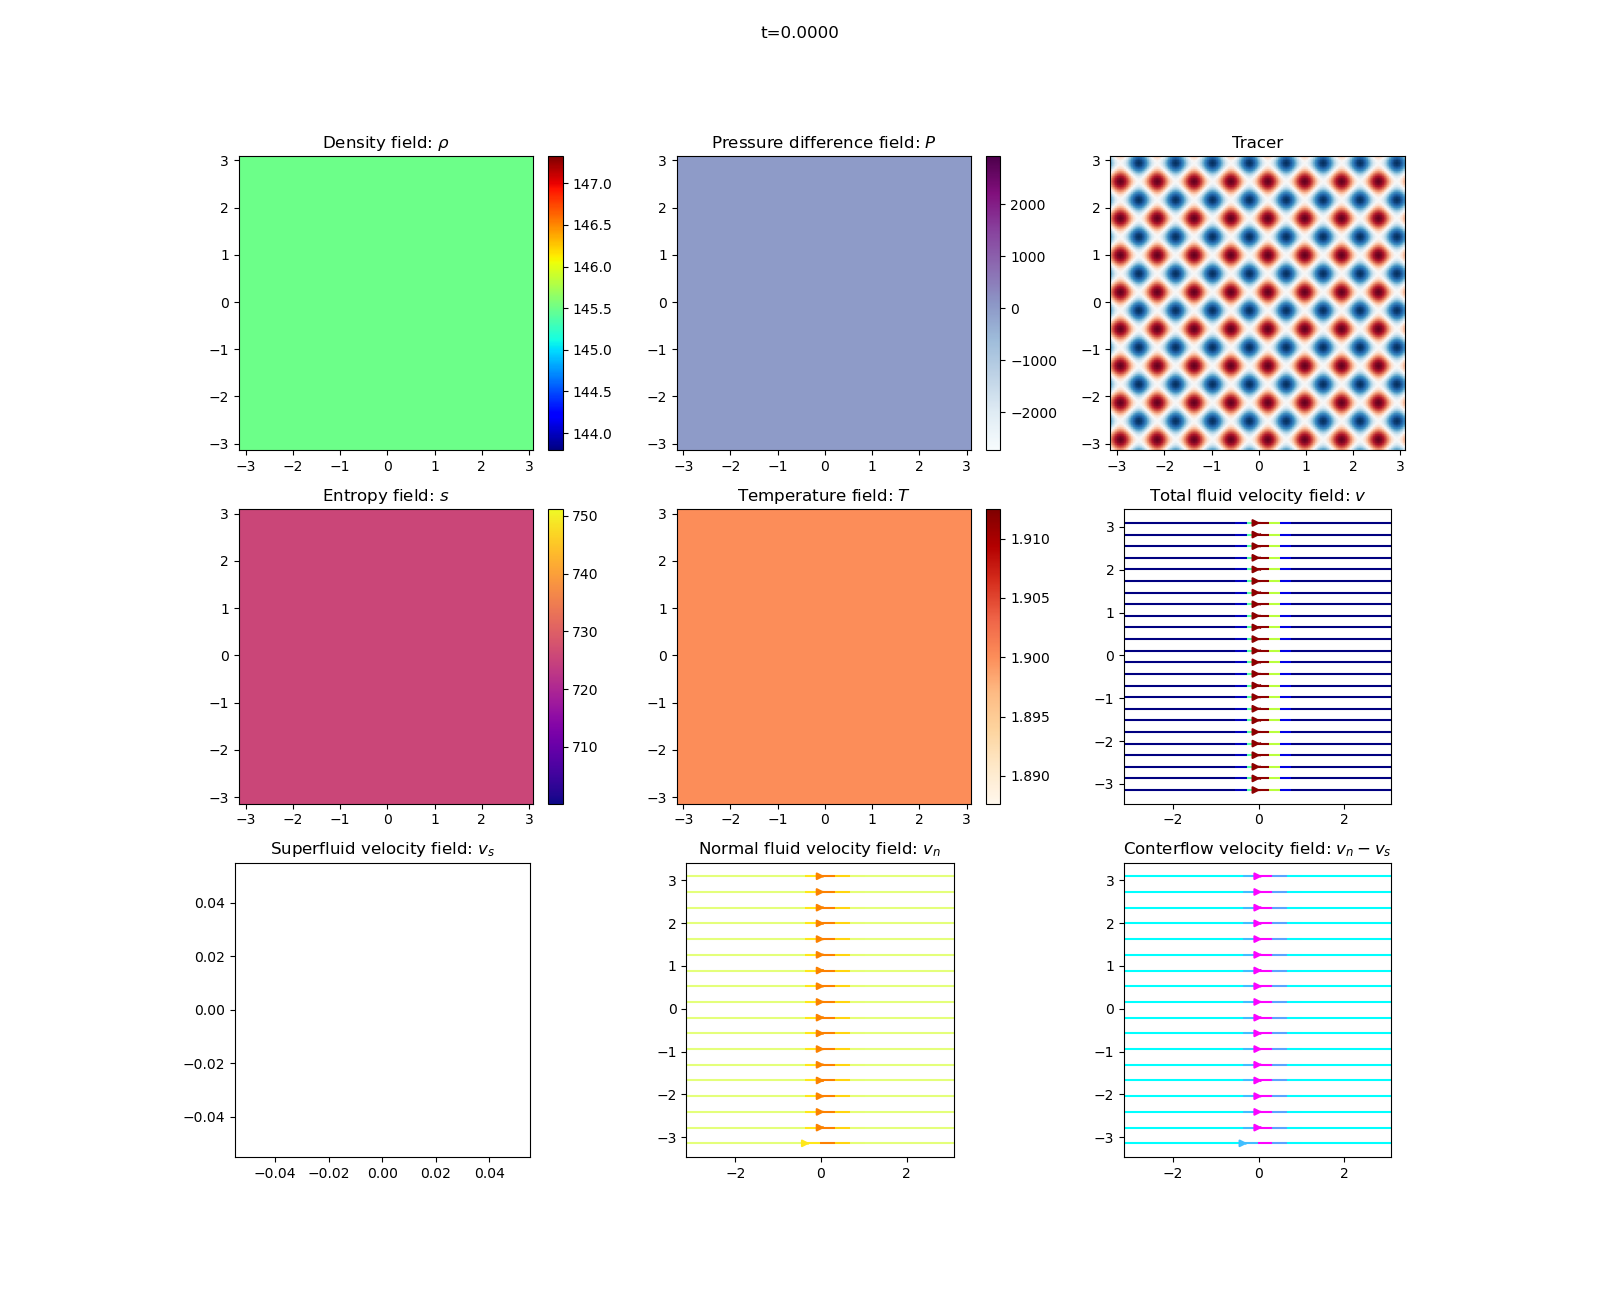
\includegraphics[width=\textwidth/3]{Sim 1/SF01_0000.png}
    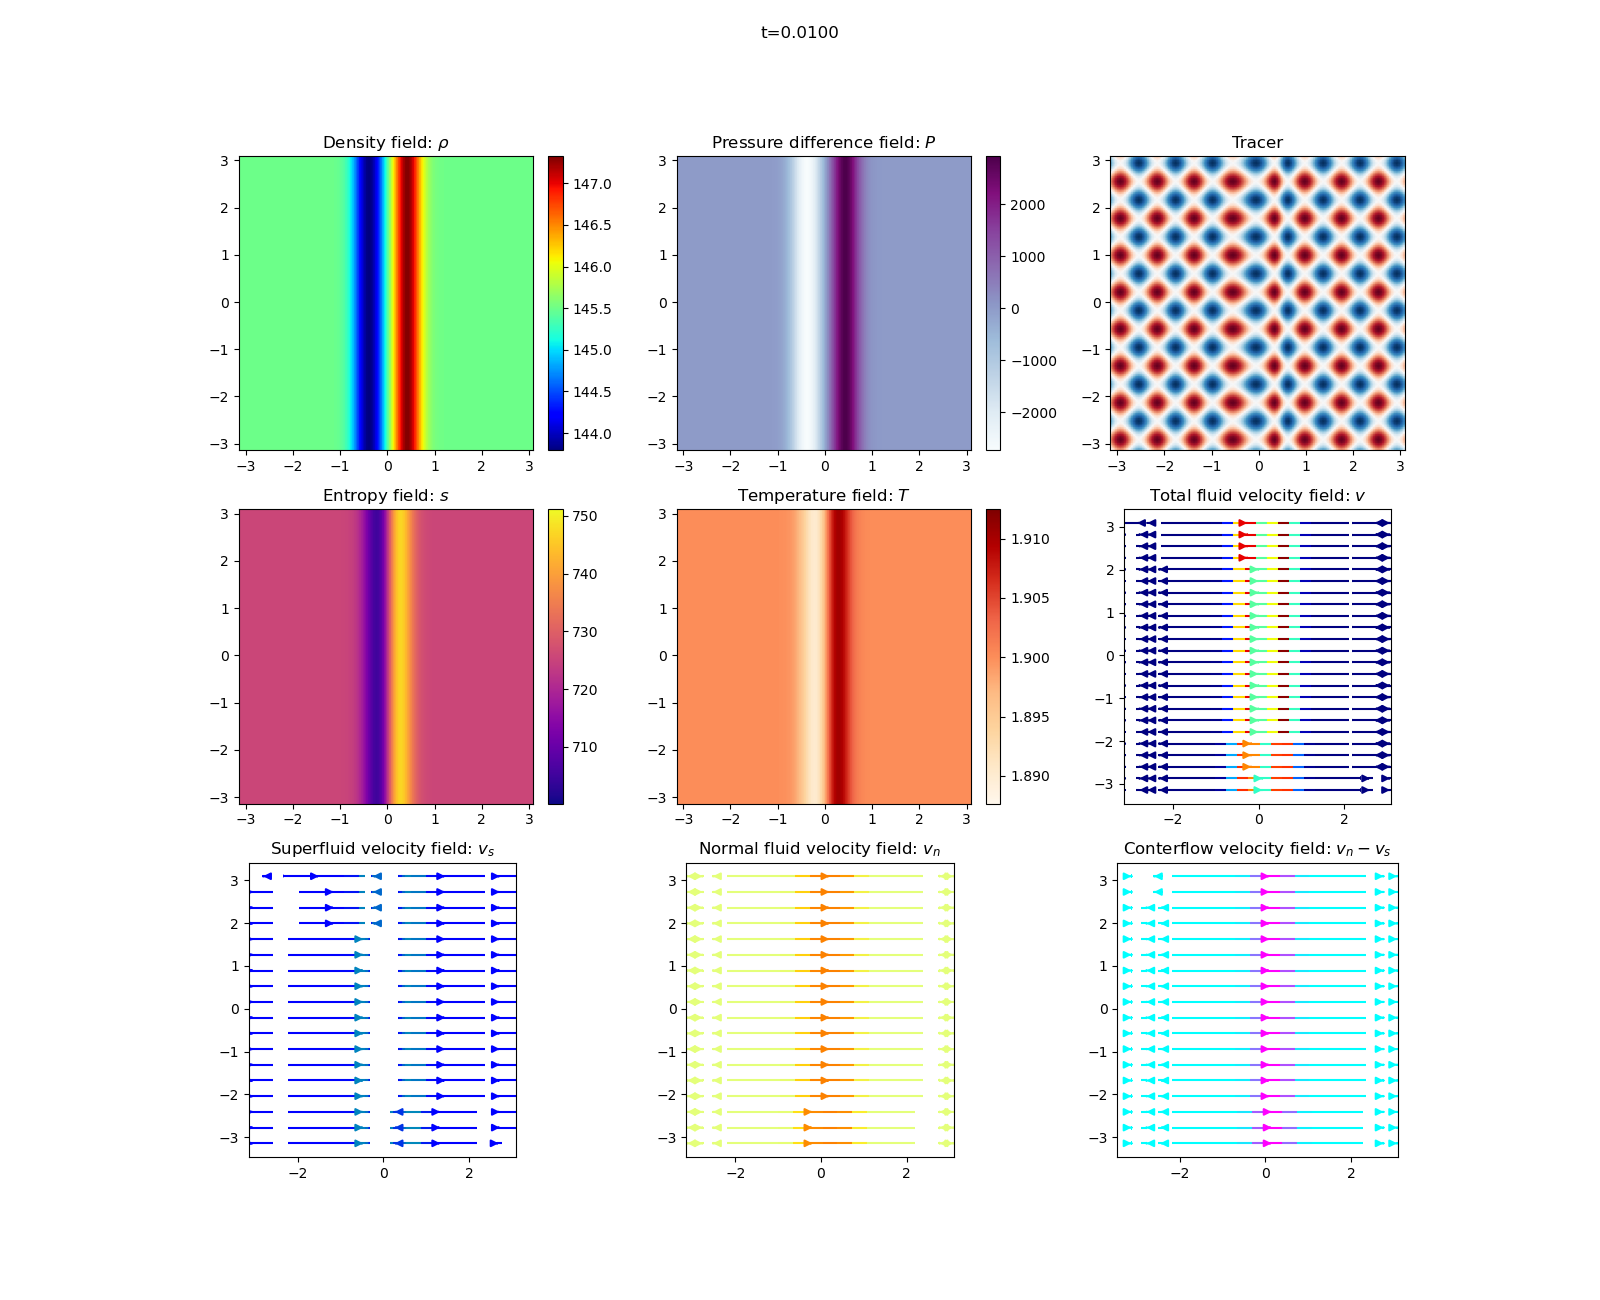
\includegraphics[width=\textwidth/3]{Sim 1/SF01_0020.png}
    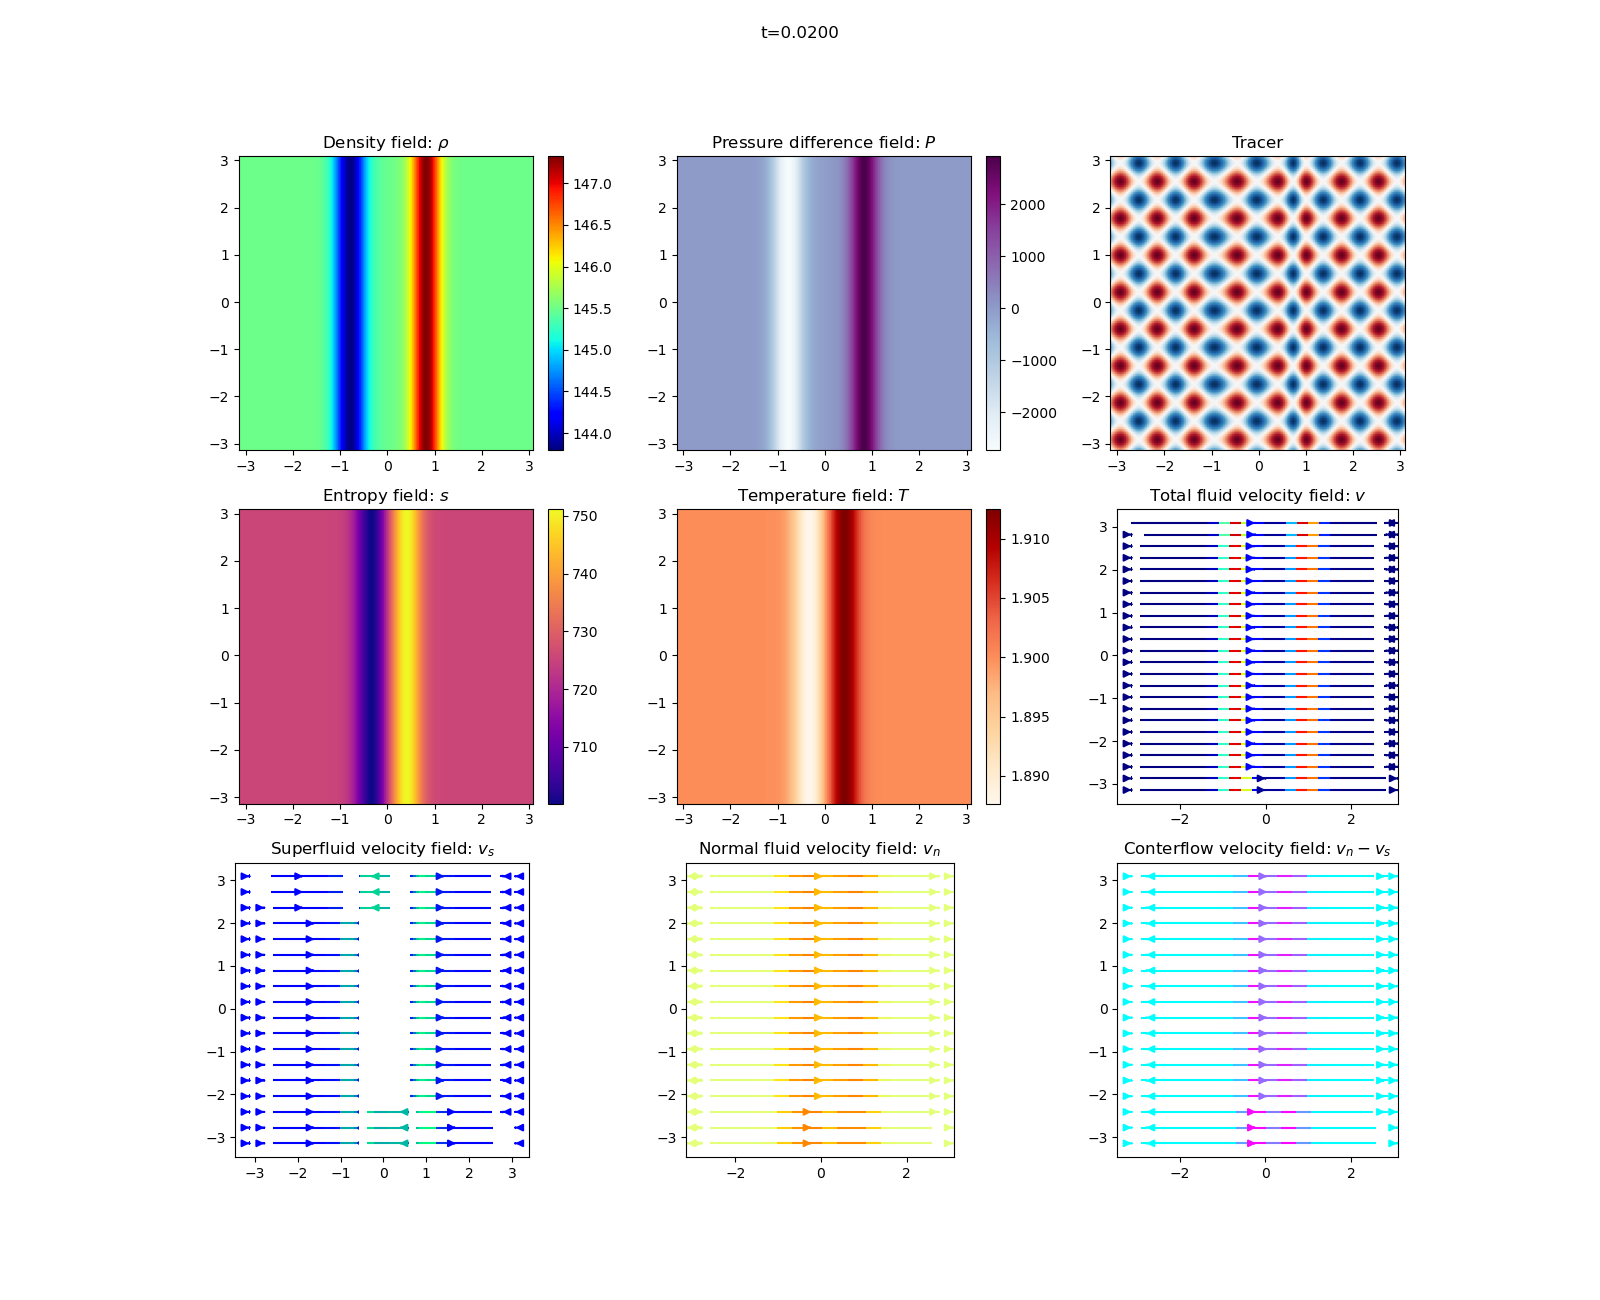
\includegraphics[width=\textwidth/3]{Sim 1/SF01_0040.png}
    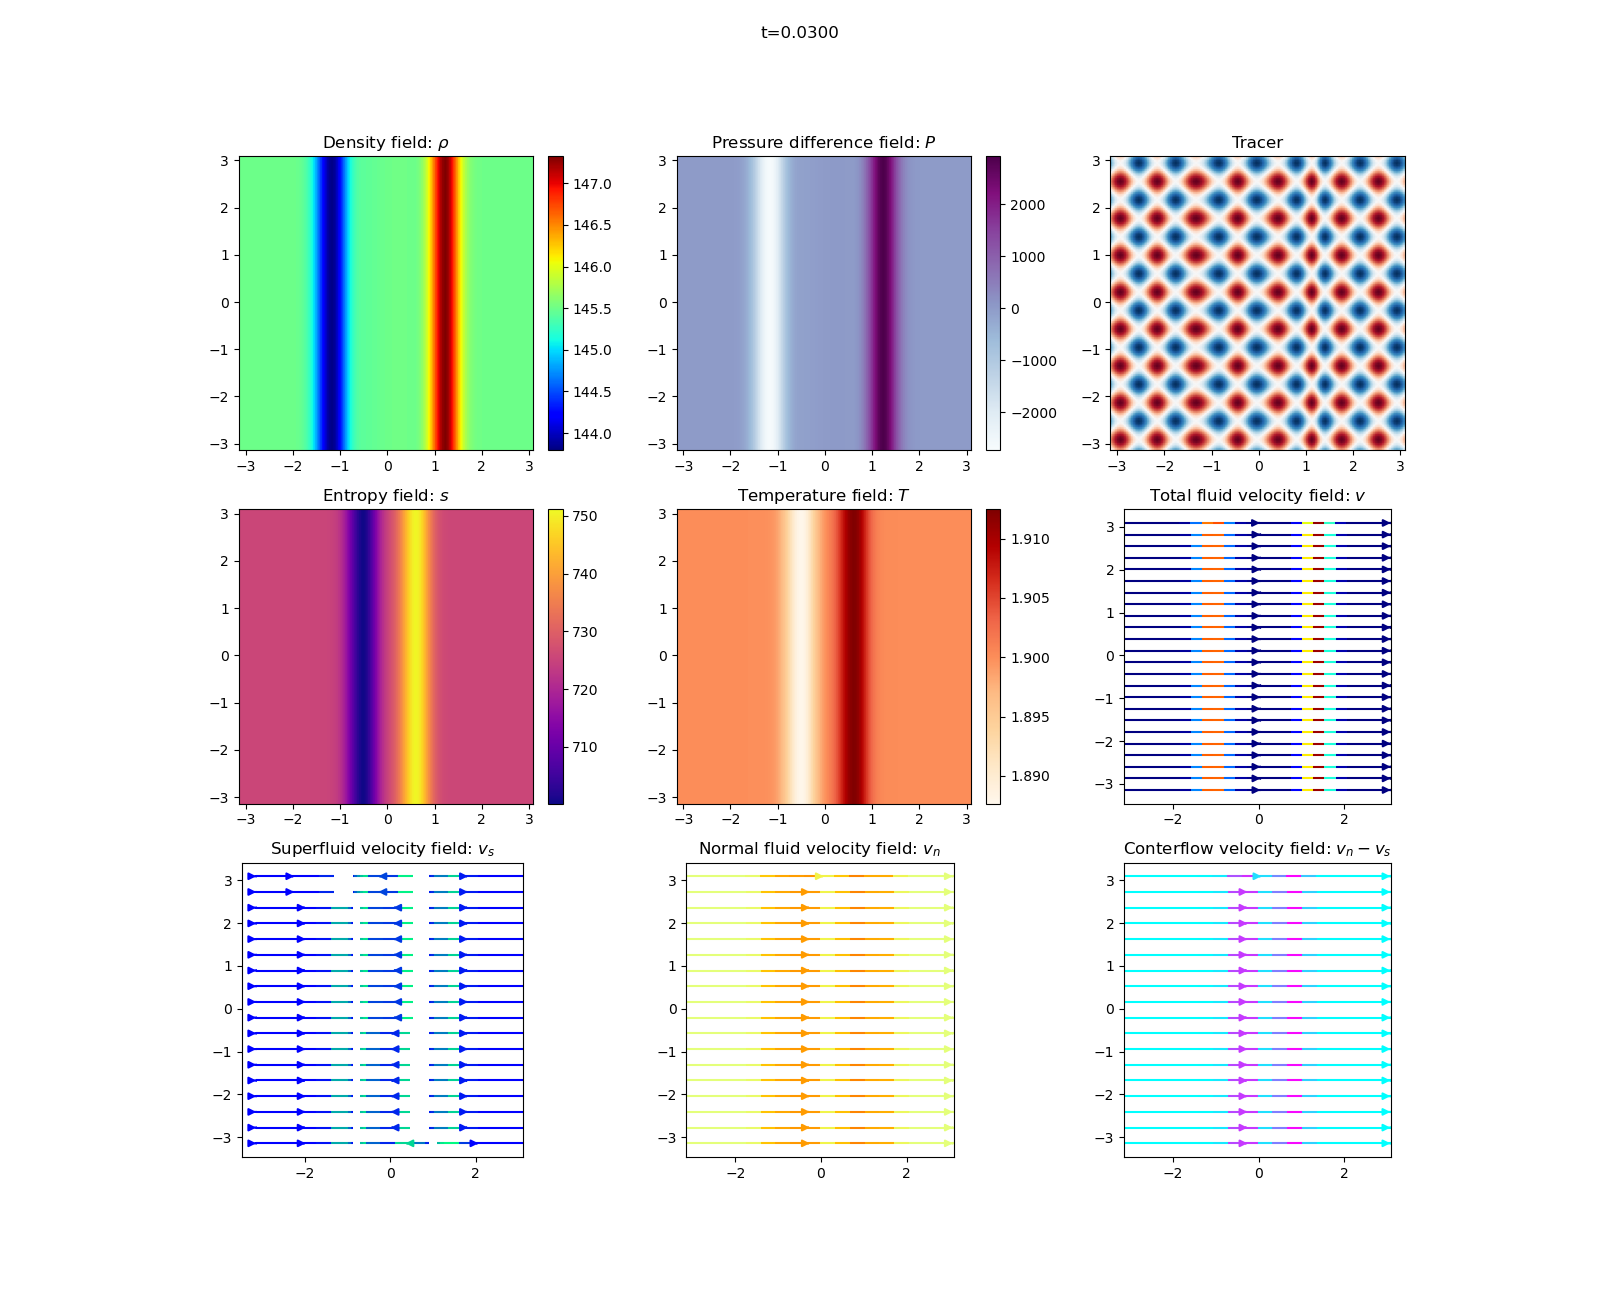
\includegraphics[width=\textwidth/3]{Sim 1/SF01_0060.png}
    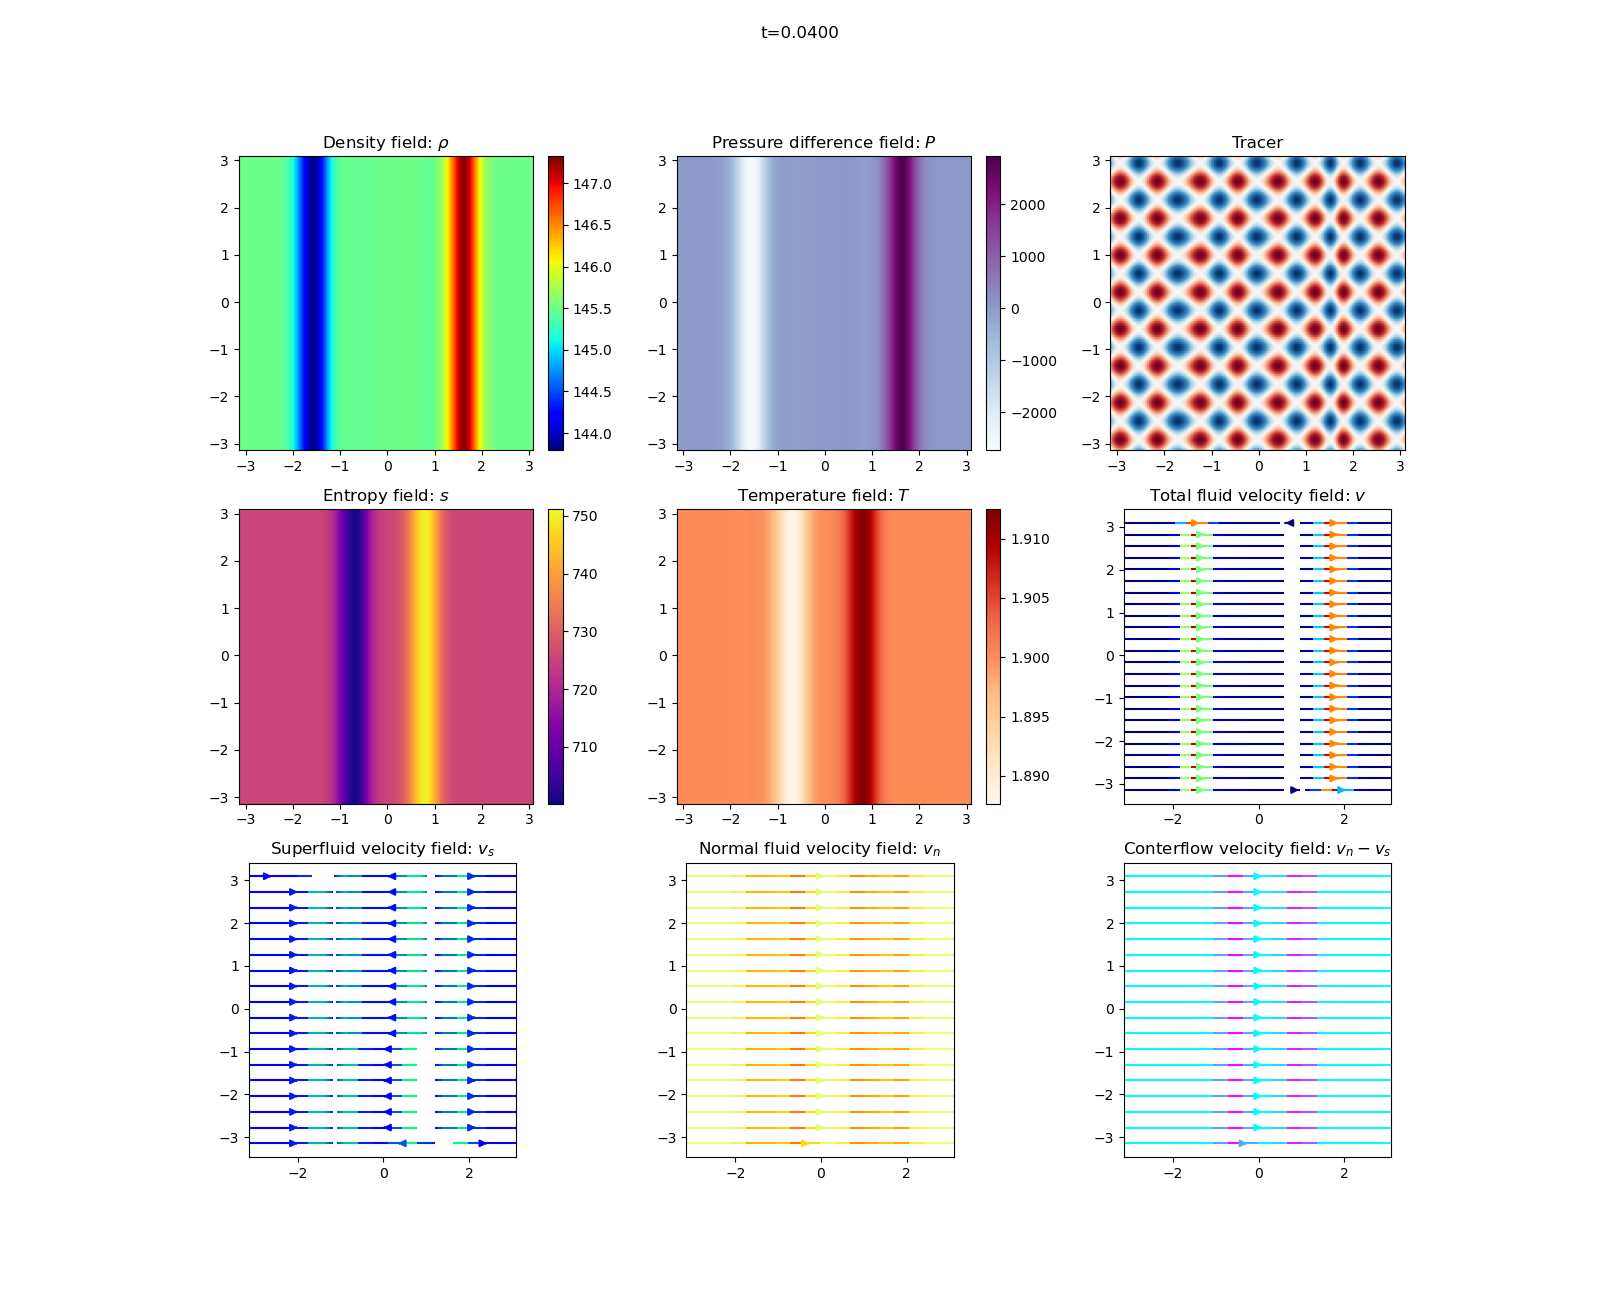
\includegraphics[width=\textwidth/3]{Sim 1/SF01_0080.png}
    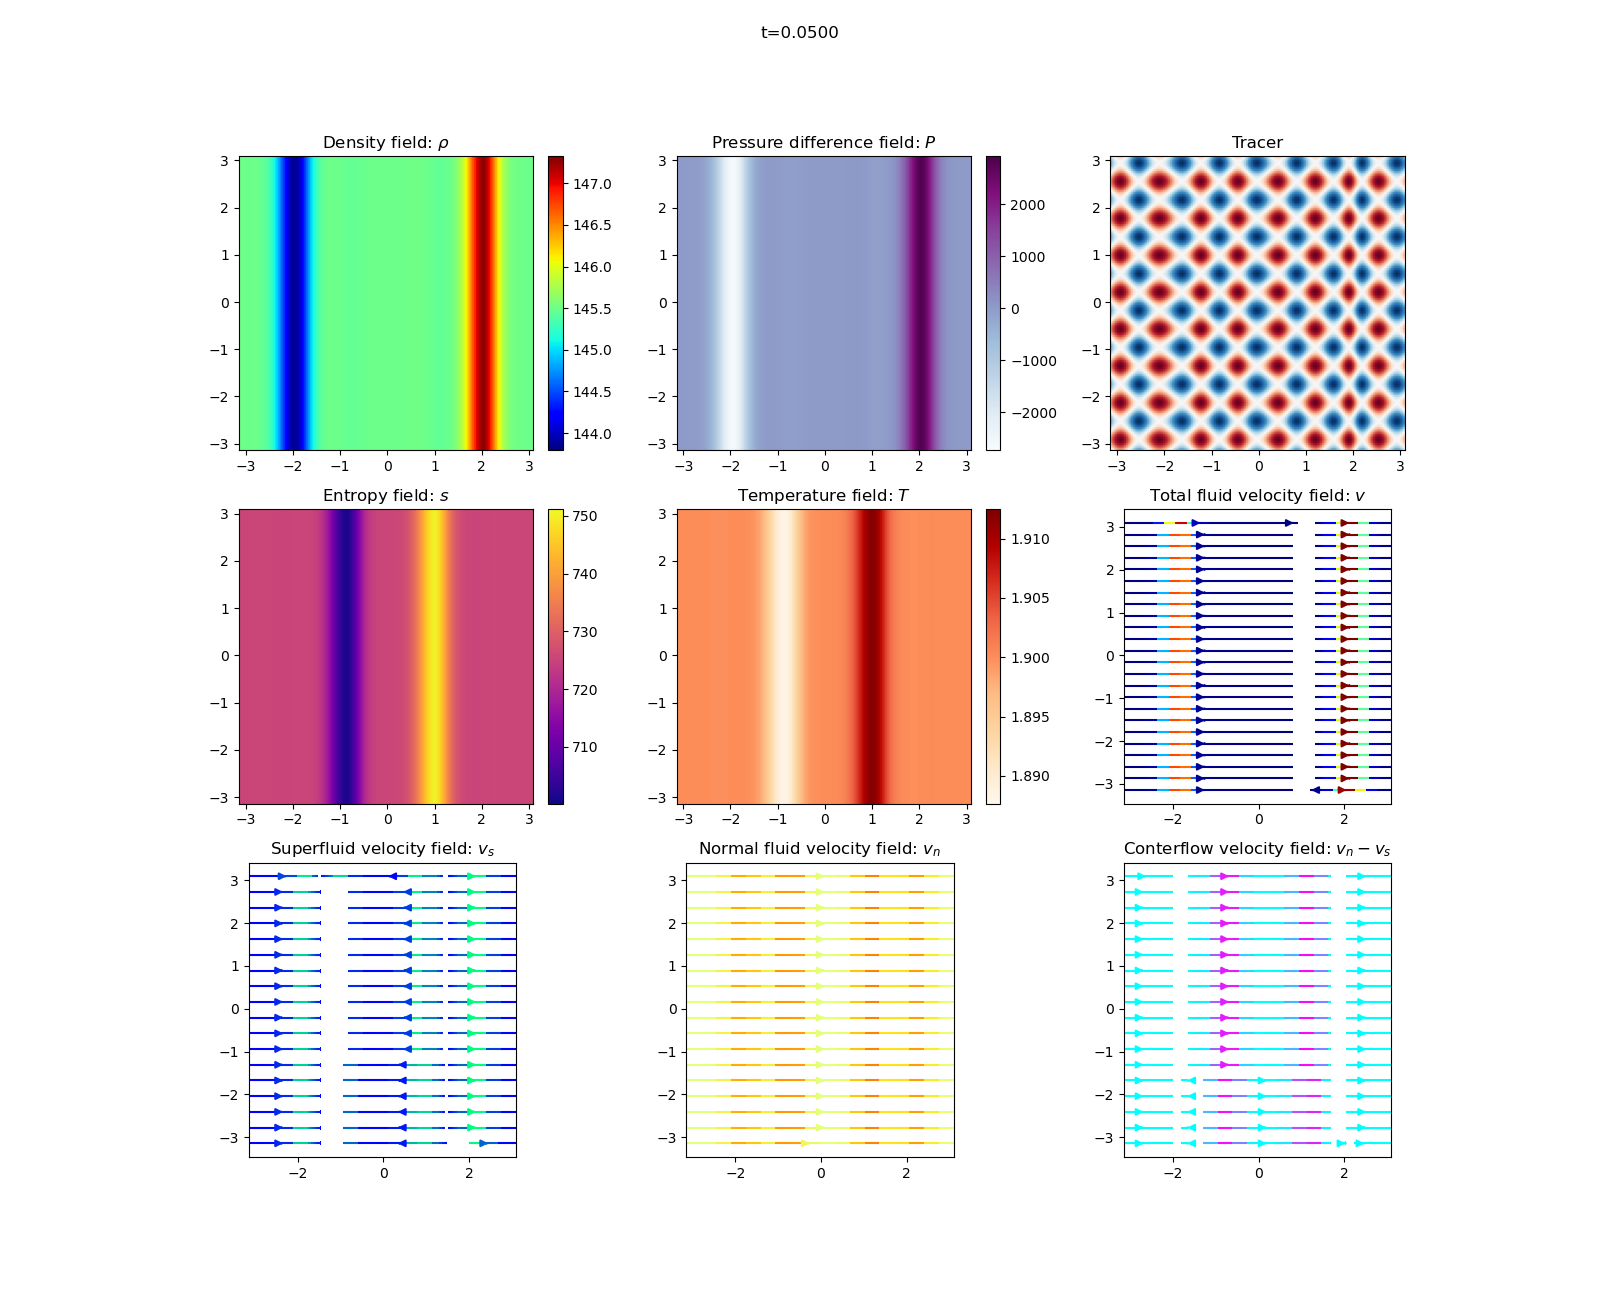
\includegraphics[width=\textwidth/3]{Sim 1/SF01_0100.png}
    \caption{Snapshots from simulation 1}
    \label{sim1}
\end{figure}

\subsubsection{Simulation 2}
In the next two simulations we will explore what happens when we add a perturbation to the density or entropy field.
In simulation 2 we set the initial density to \(\rho = \rho_0 + e^{-10x^2}\) and we bserved how this perturbation inthe density field crates a perturbation in the entropy field as can be seen in figure \ref{sim2_start}.

\begin{figure}[h]
    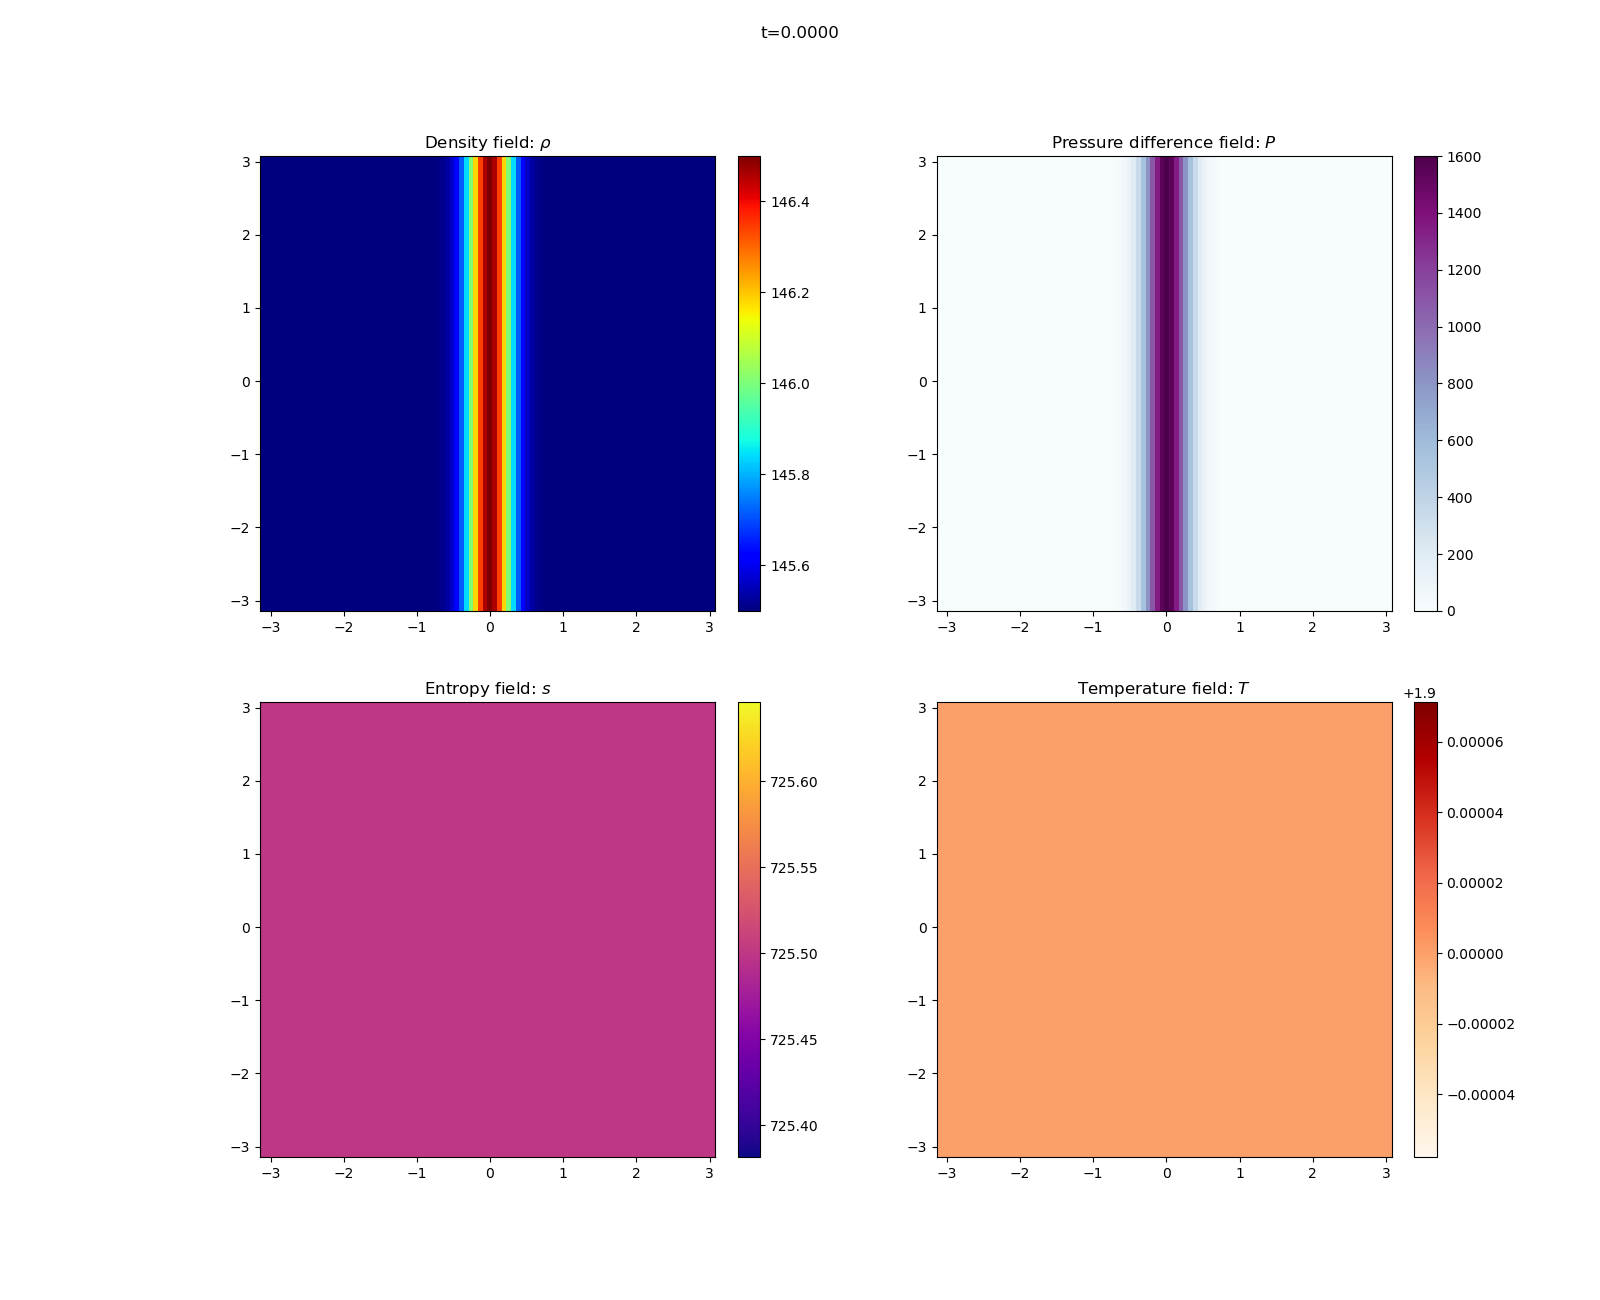
\includegraphics[width=\textwidth/3]{Sim 2/SF02_0000.png}
    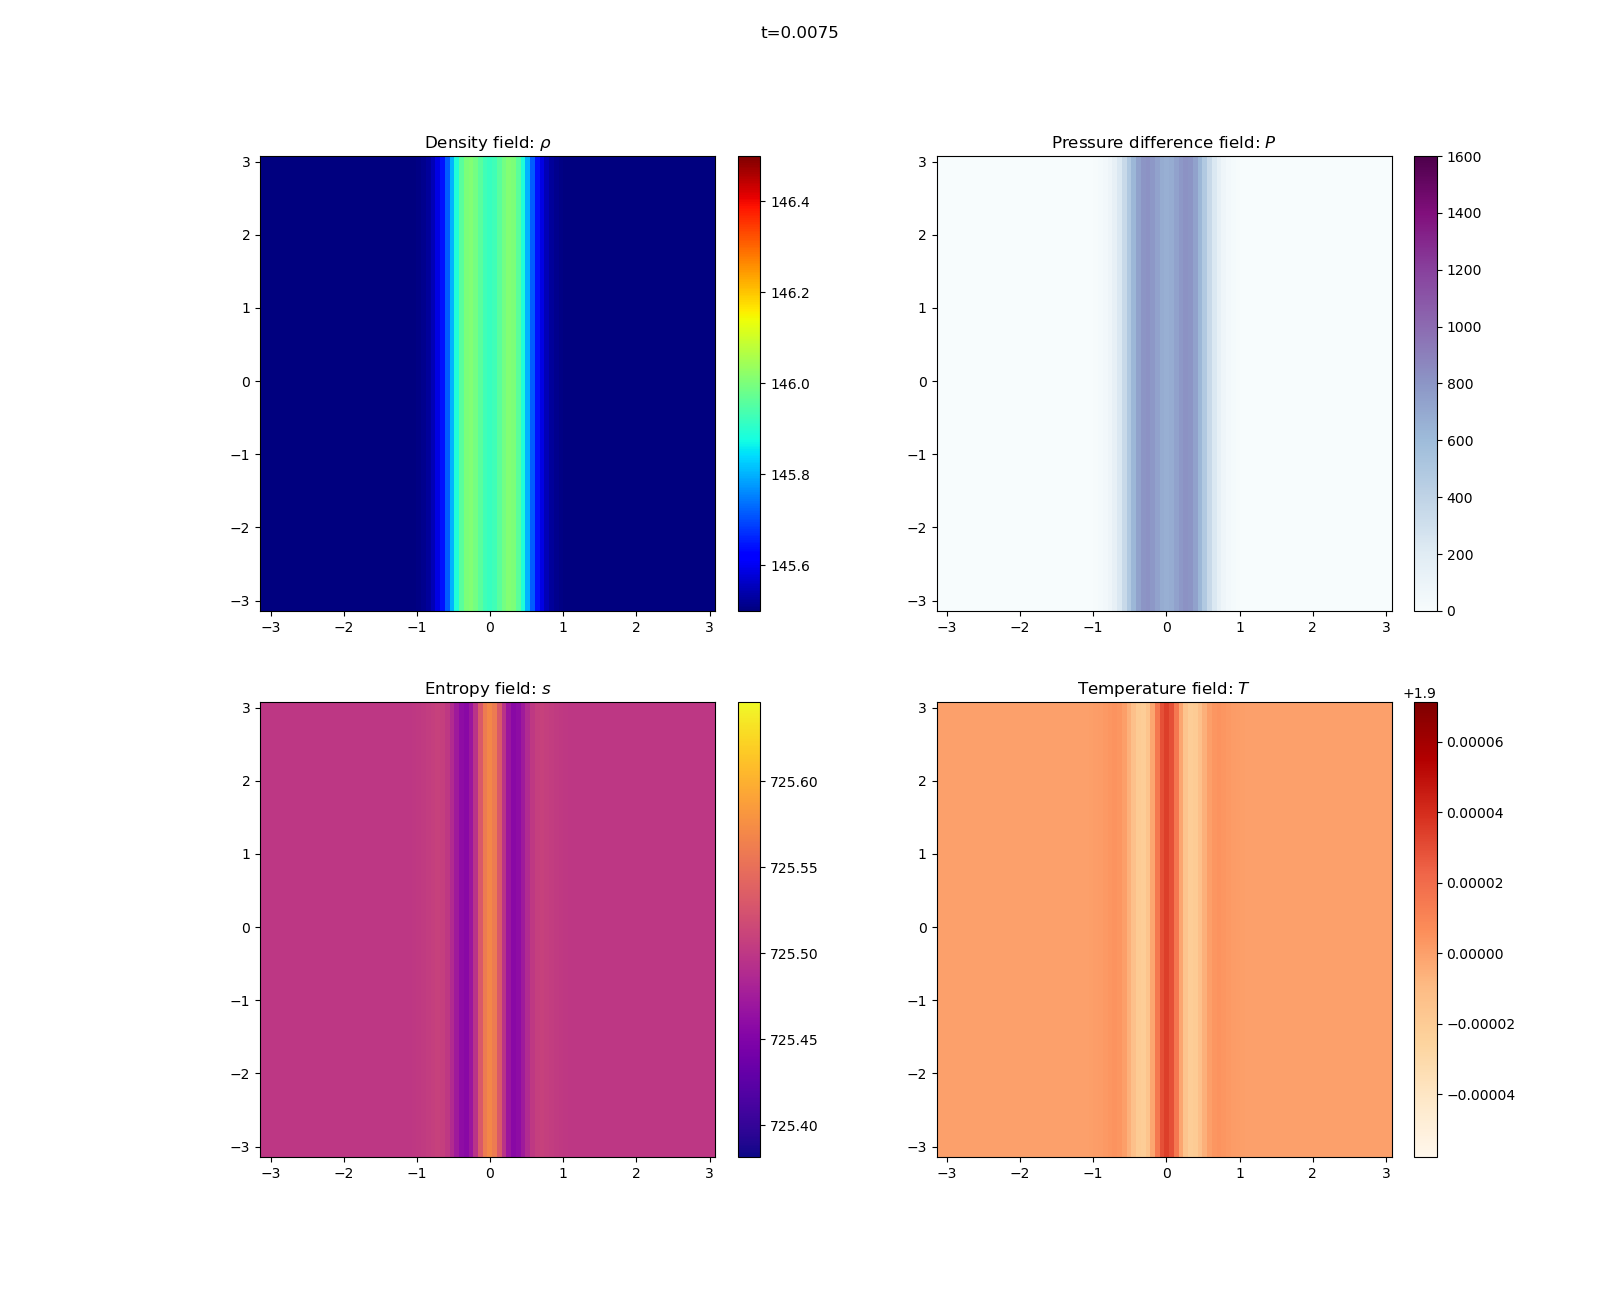
\includegraphics[width=\textwidth/3]{Sim 2/SF02_0003.png}
    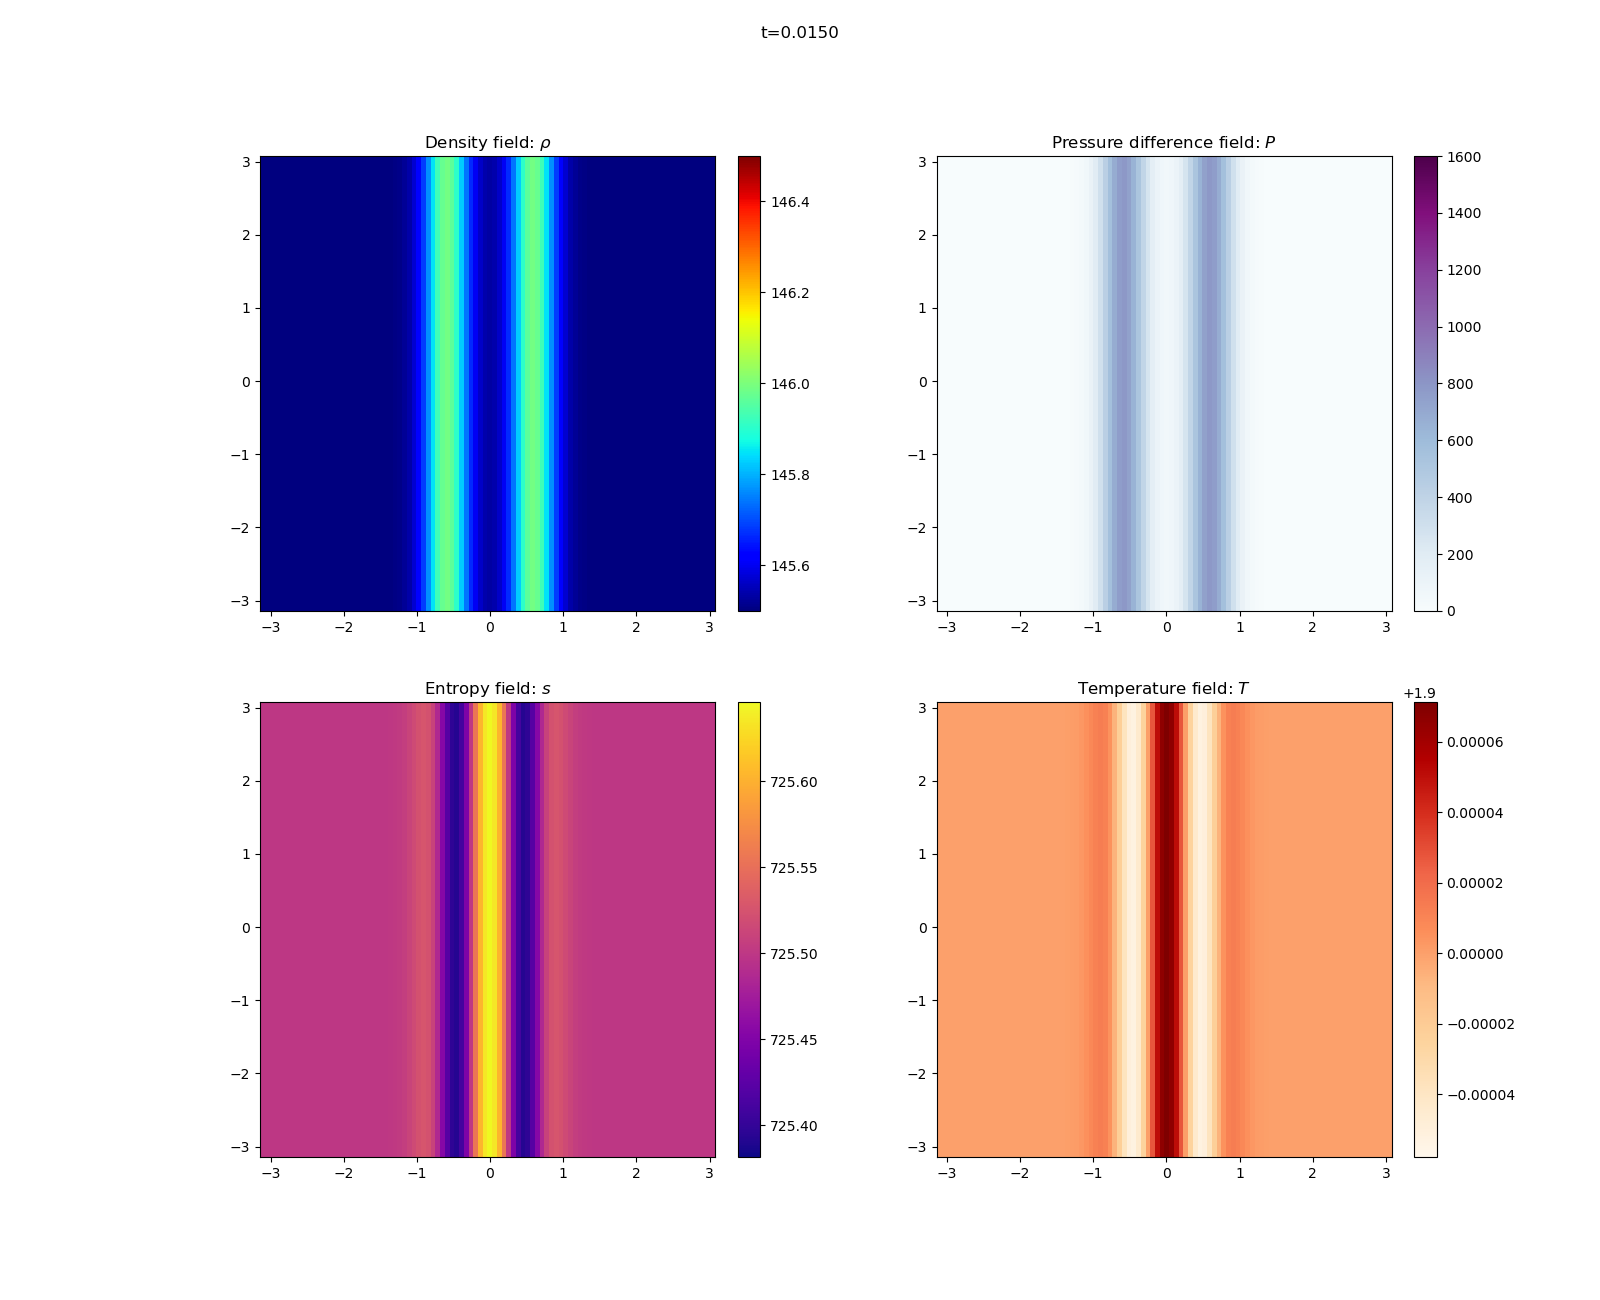
\includegraphics[width=\textwidth/3]{Sim 2/SF02_0006.png}
    \caption{Snapshots from simulation 2}
    \label{sim2_start}
\end{figure}

In figure \ref{sim2} we observe two waves in the entropy field, one that follows the wave in the density field, and another one that falls behind.

\begin{figure}[h]
    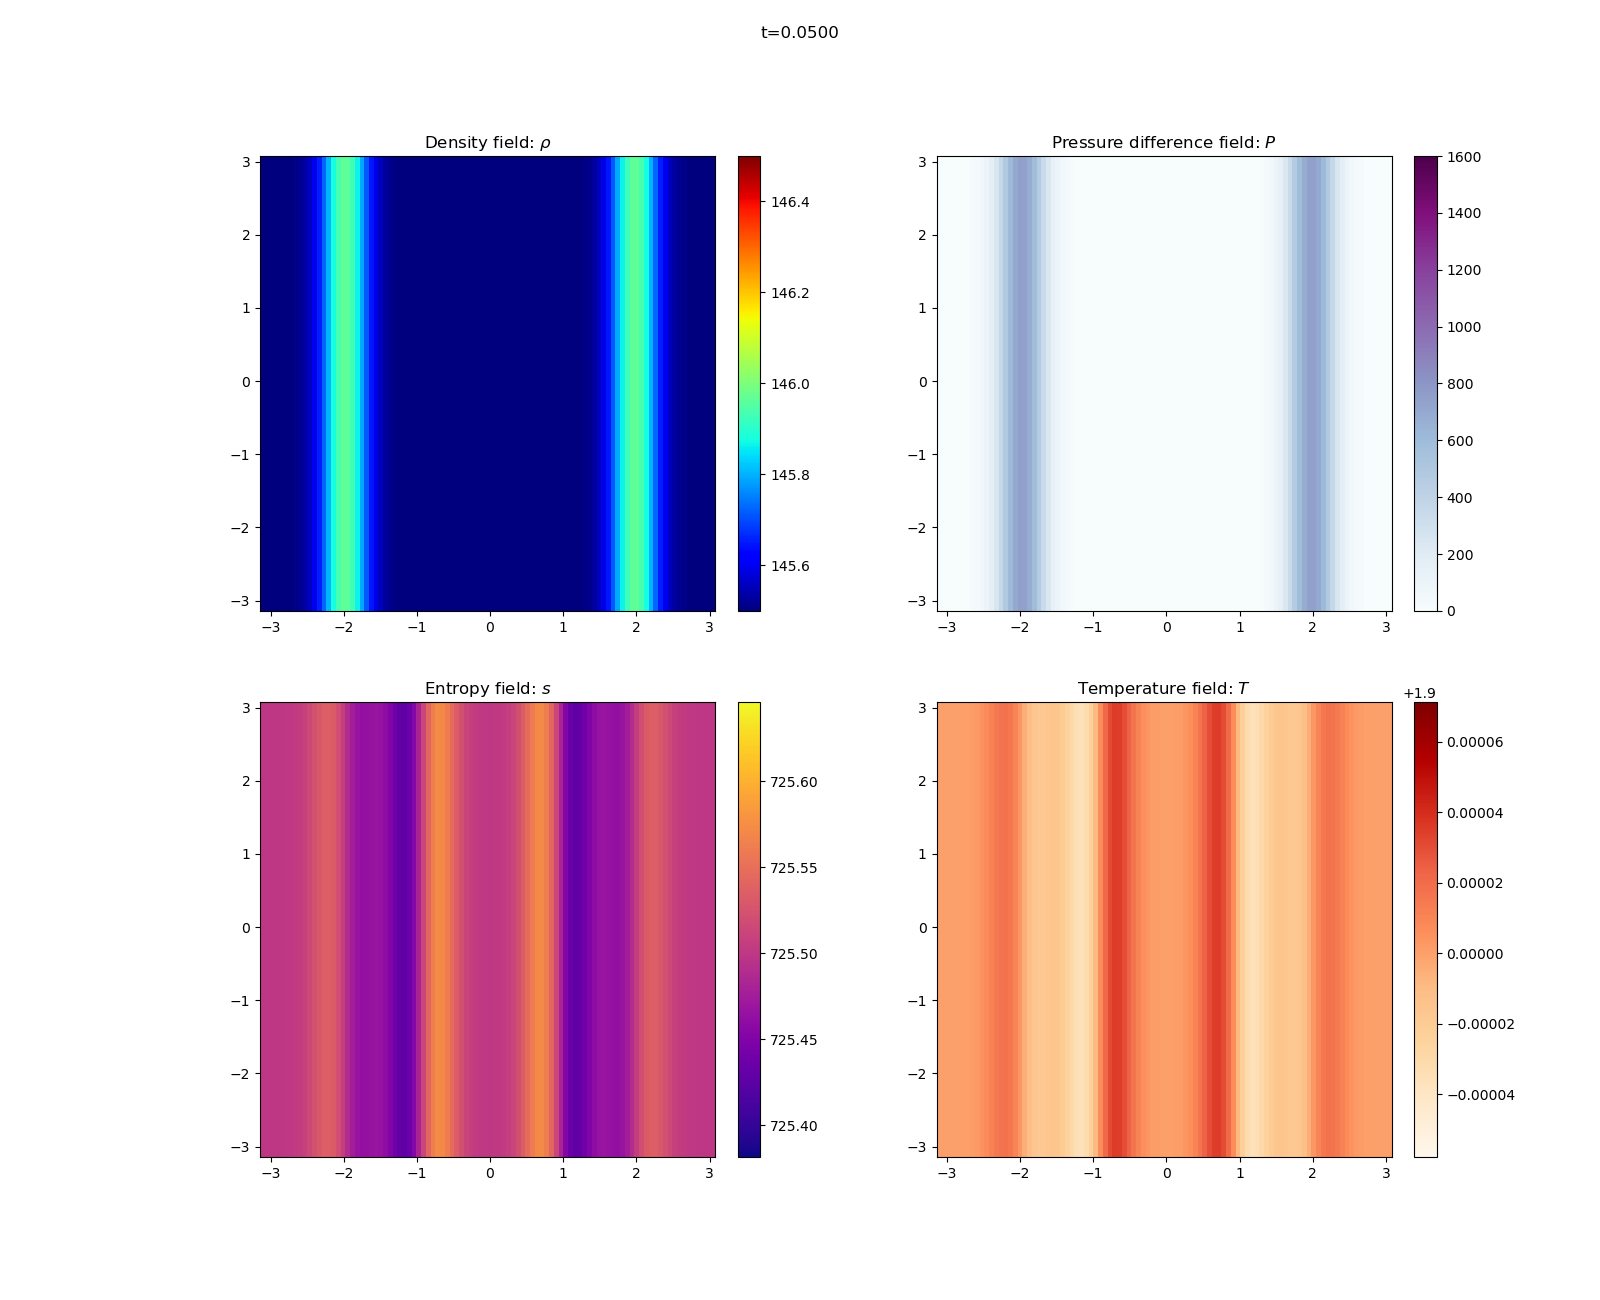
\includegraphics[width=\textwidth/3]{Sim 2/SF02_0020.png}
    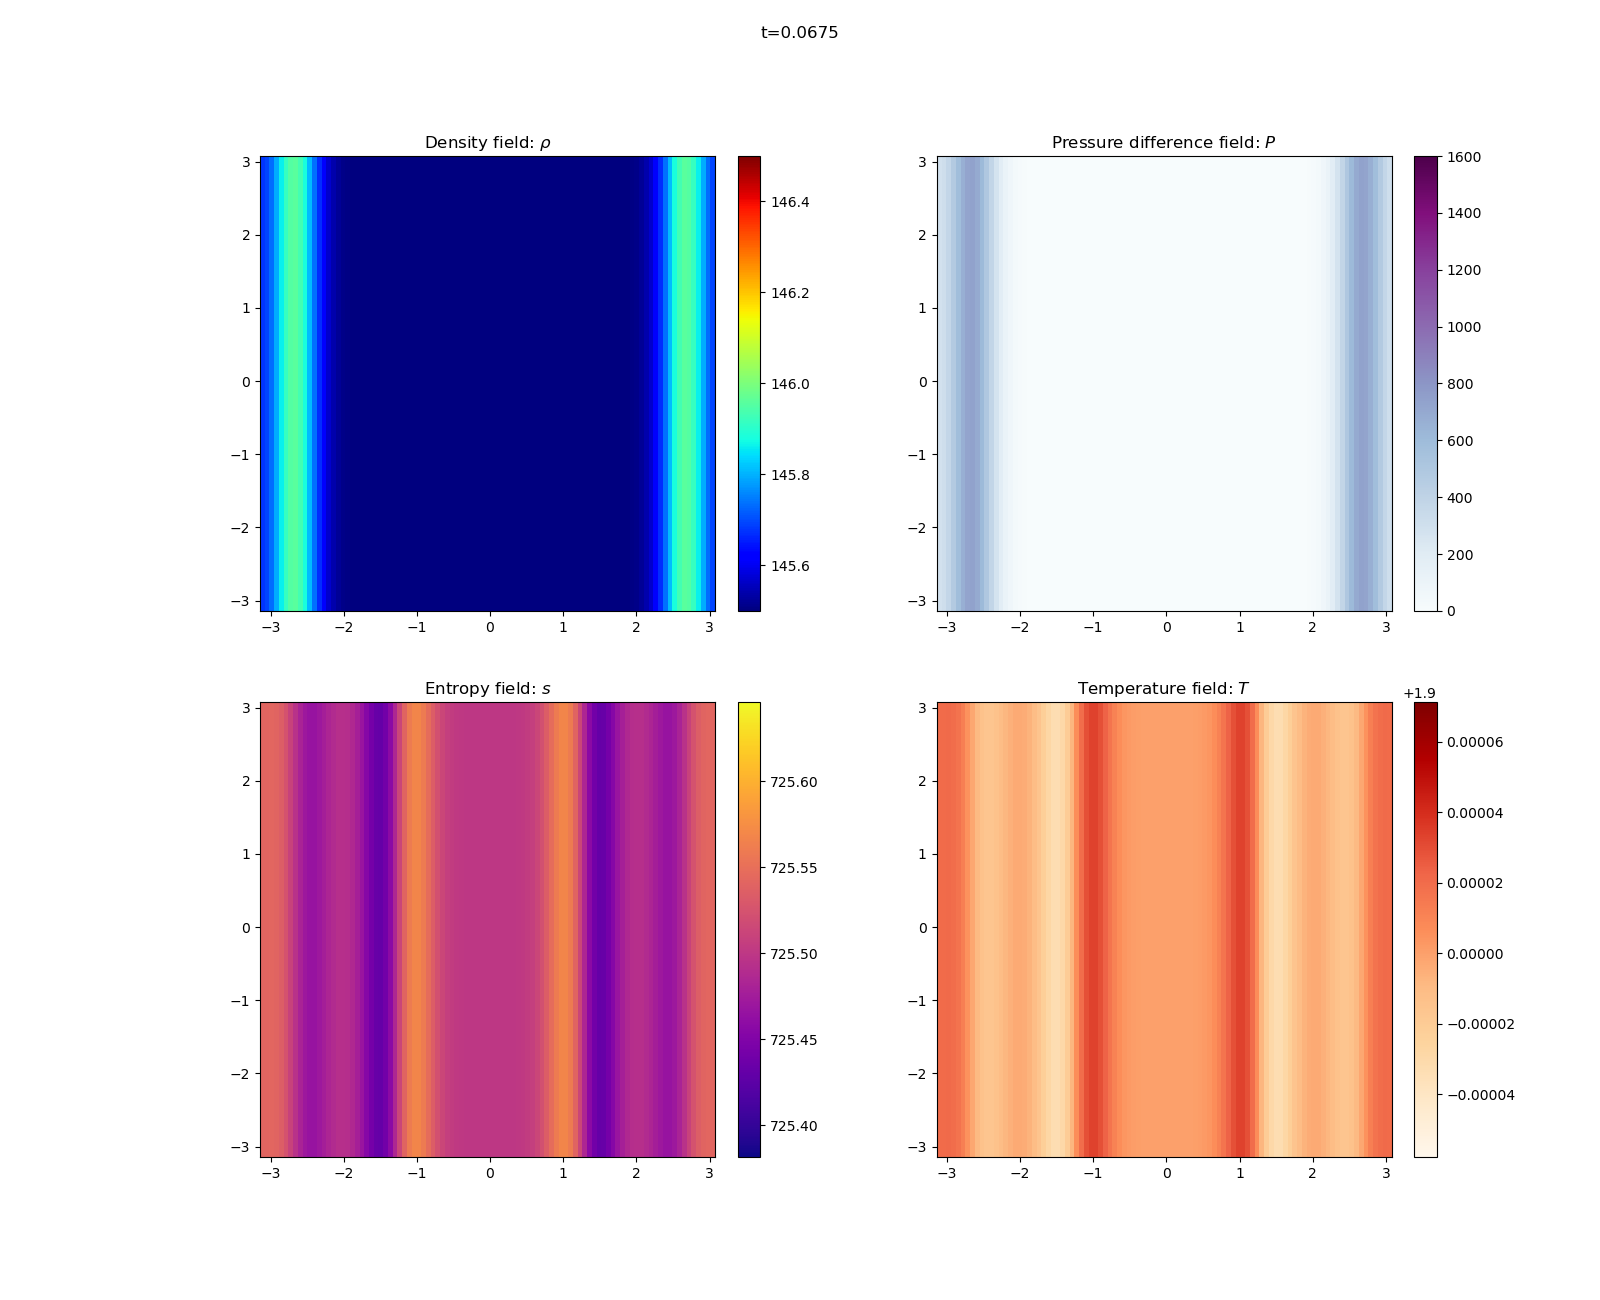
\includegraphics[width=\textwidth/3]{Sim 2/SF02_0027.png}
    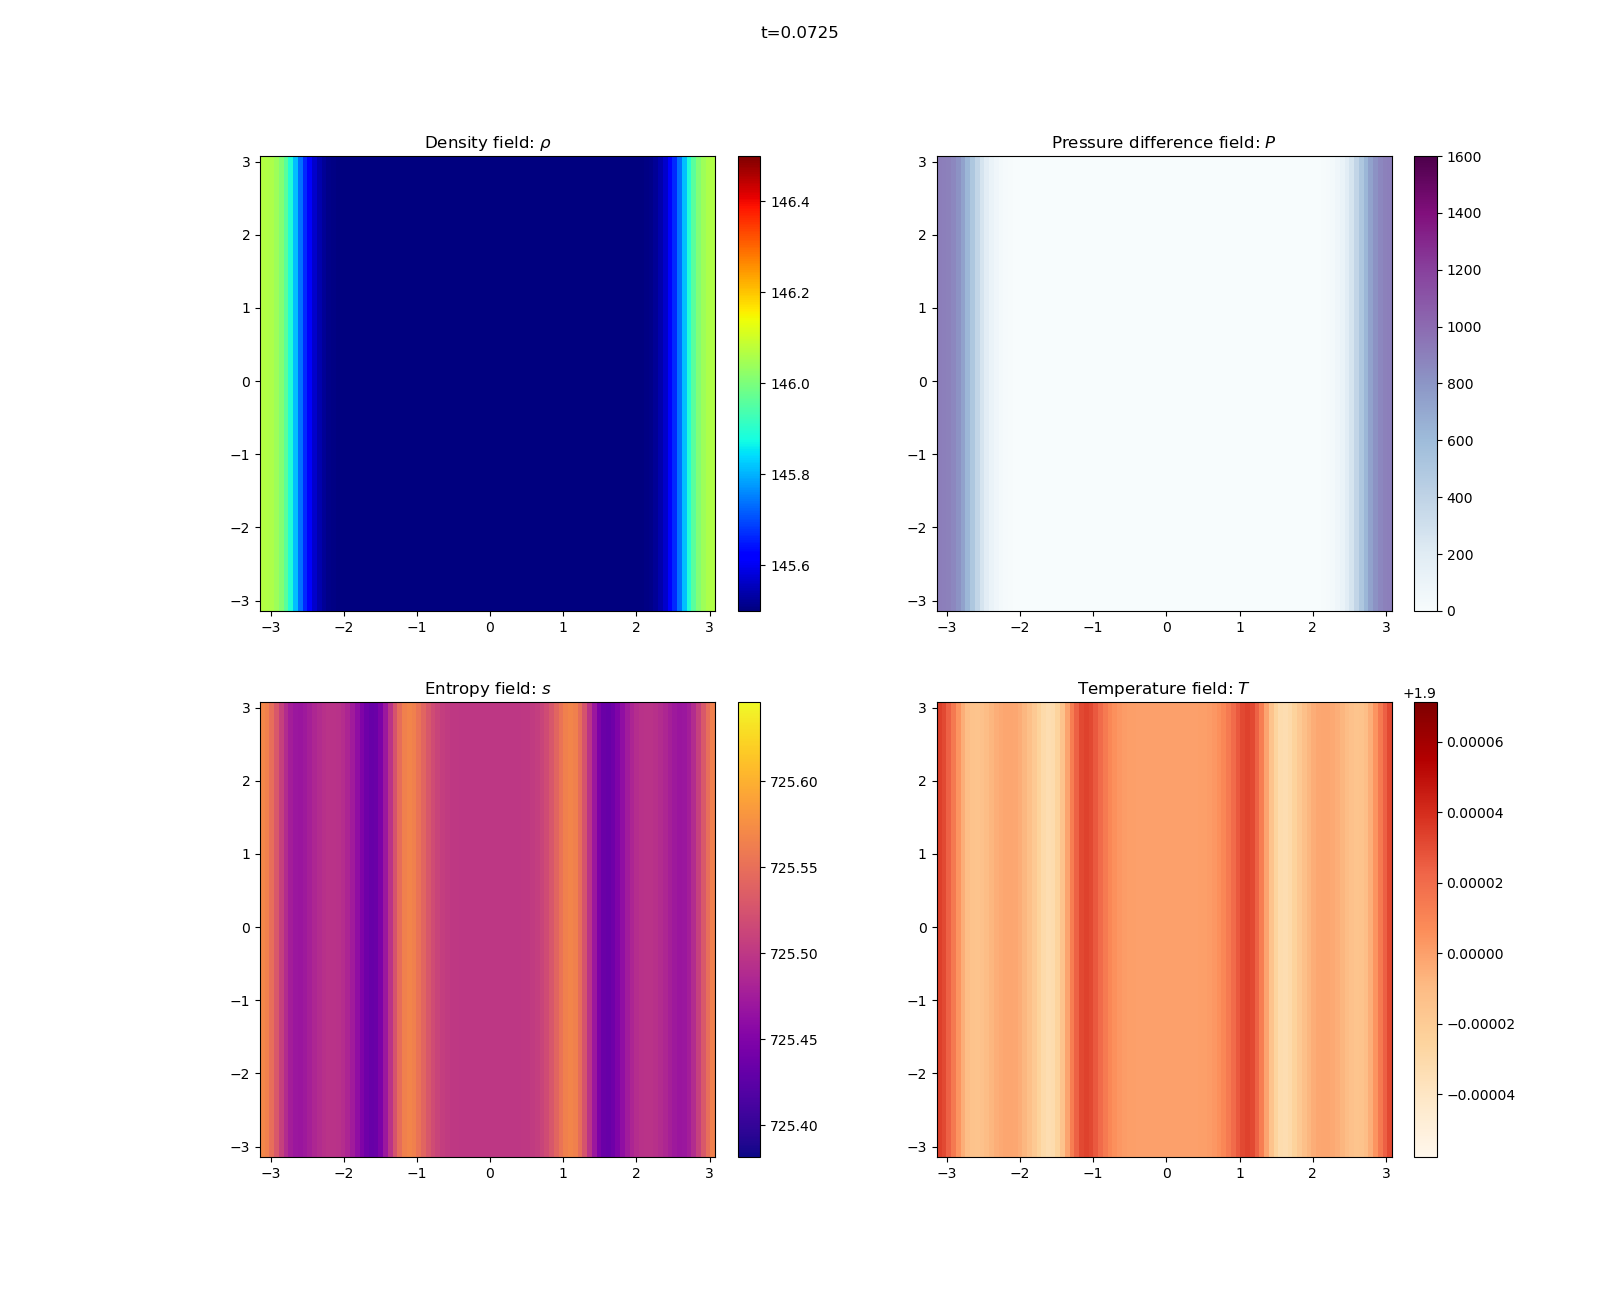
\includegraphics[width=\textwidth/3]{Sim 2/SF02_0029.png}
    \caption{Snapshots from simulation 2}
    \label{sim2}
\end{figure}

\subsubsection{Simulation 3}
In simulation 3 we set the initial entropy to \(s = s_0 + e^{-10x^2}\).
In figure \ref{sim3} we can see a similar phenomena to simulation to, in this case, there are two waves in the densiti field, one follows the entropy and the other travels faster.

\begin{figure}[h]
    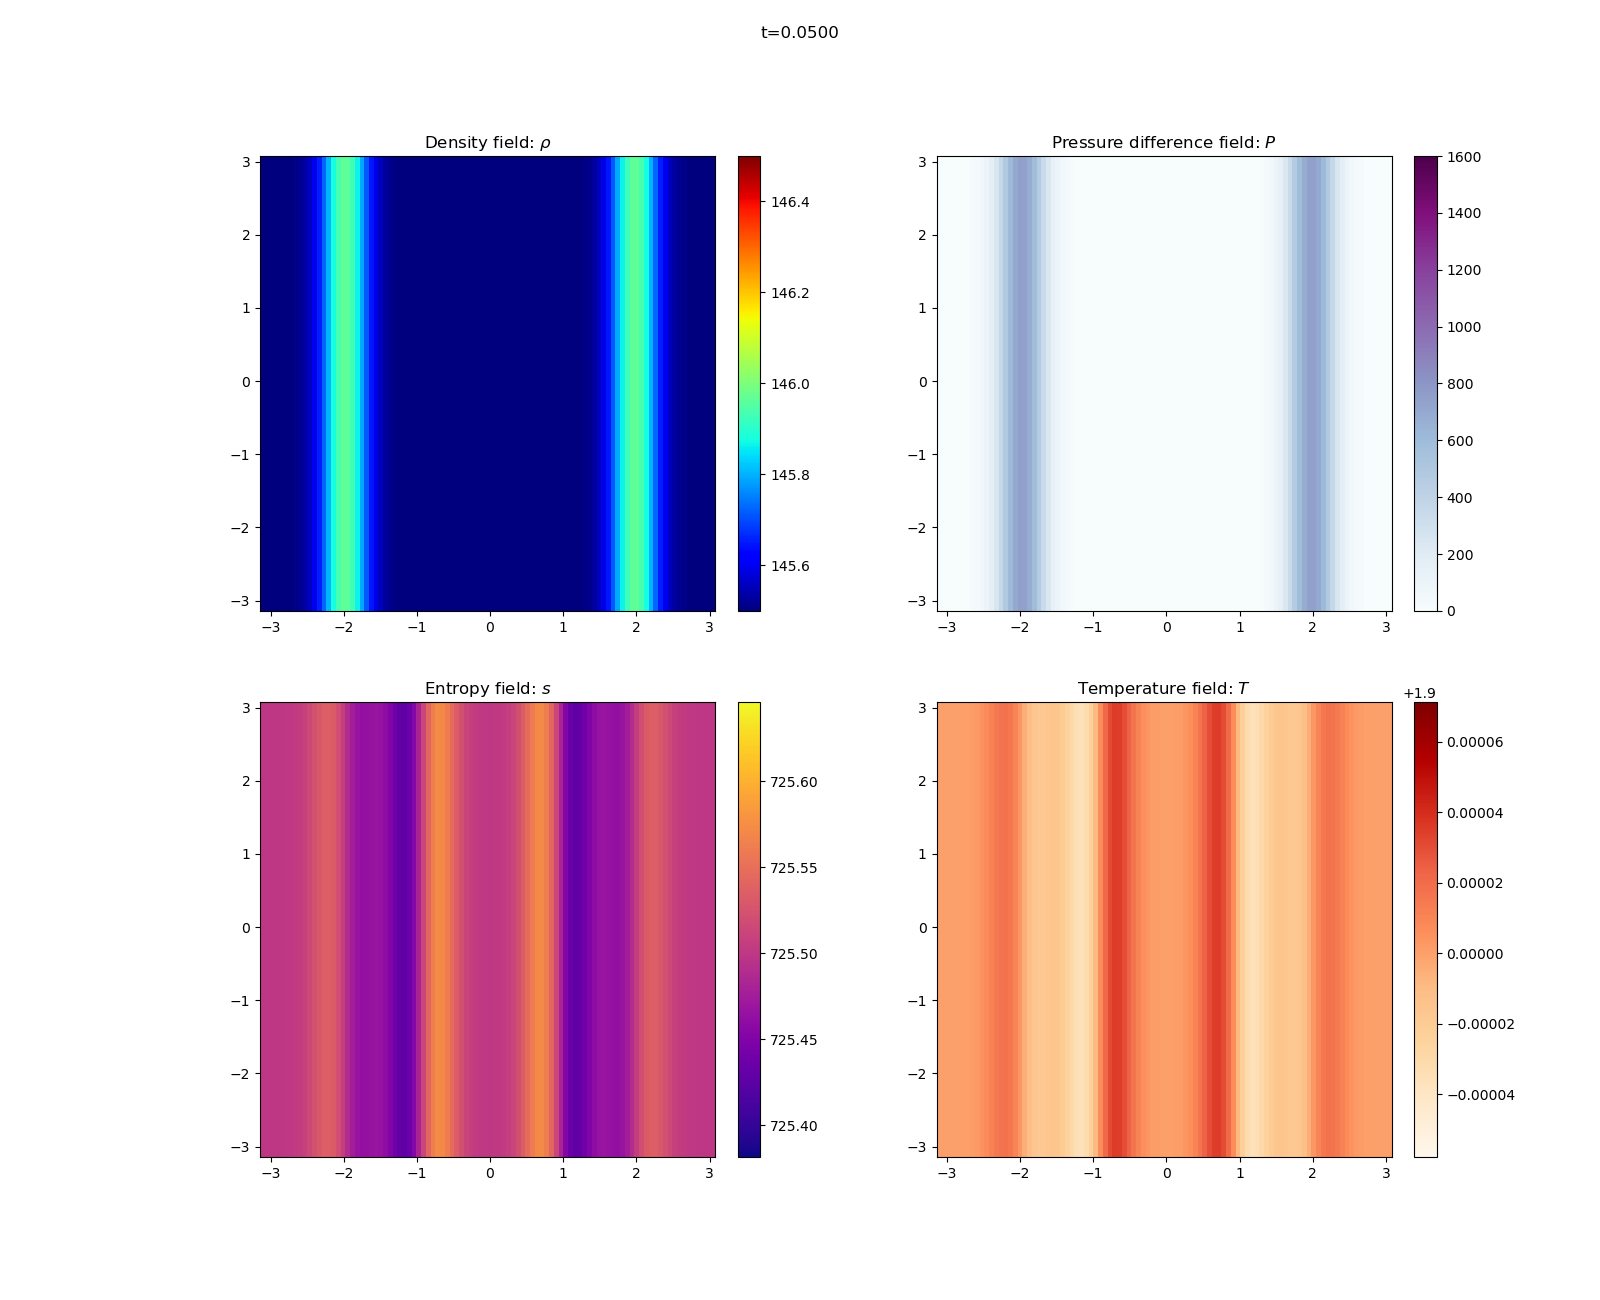
\includegraphics[width=\textwidth/3]{Sim 2/SF02_0020.png}
    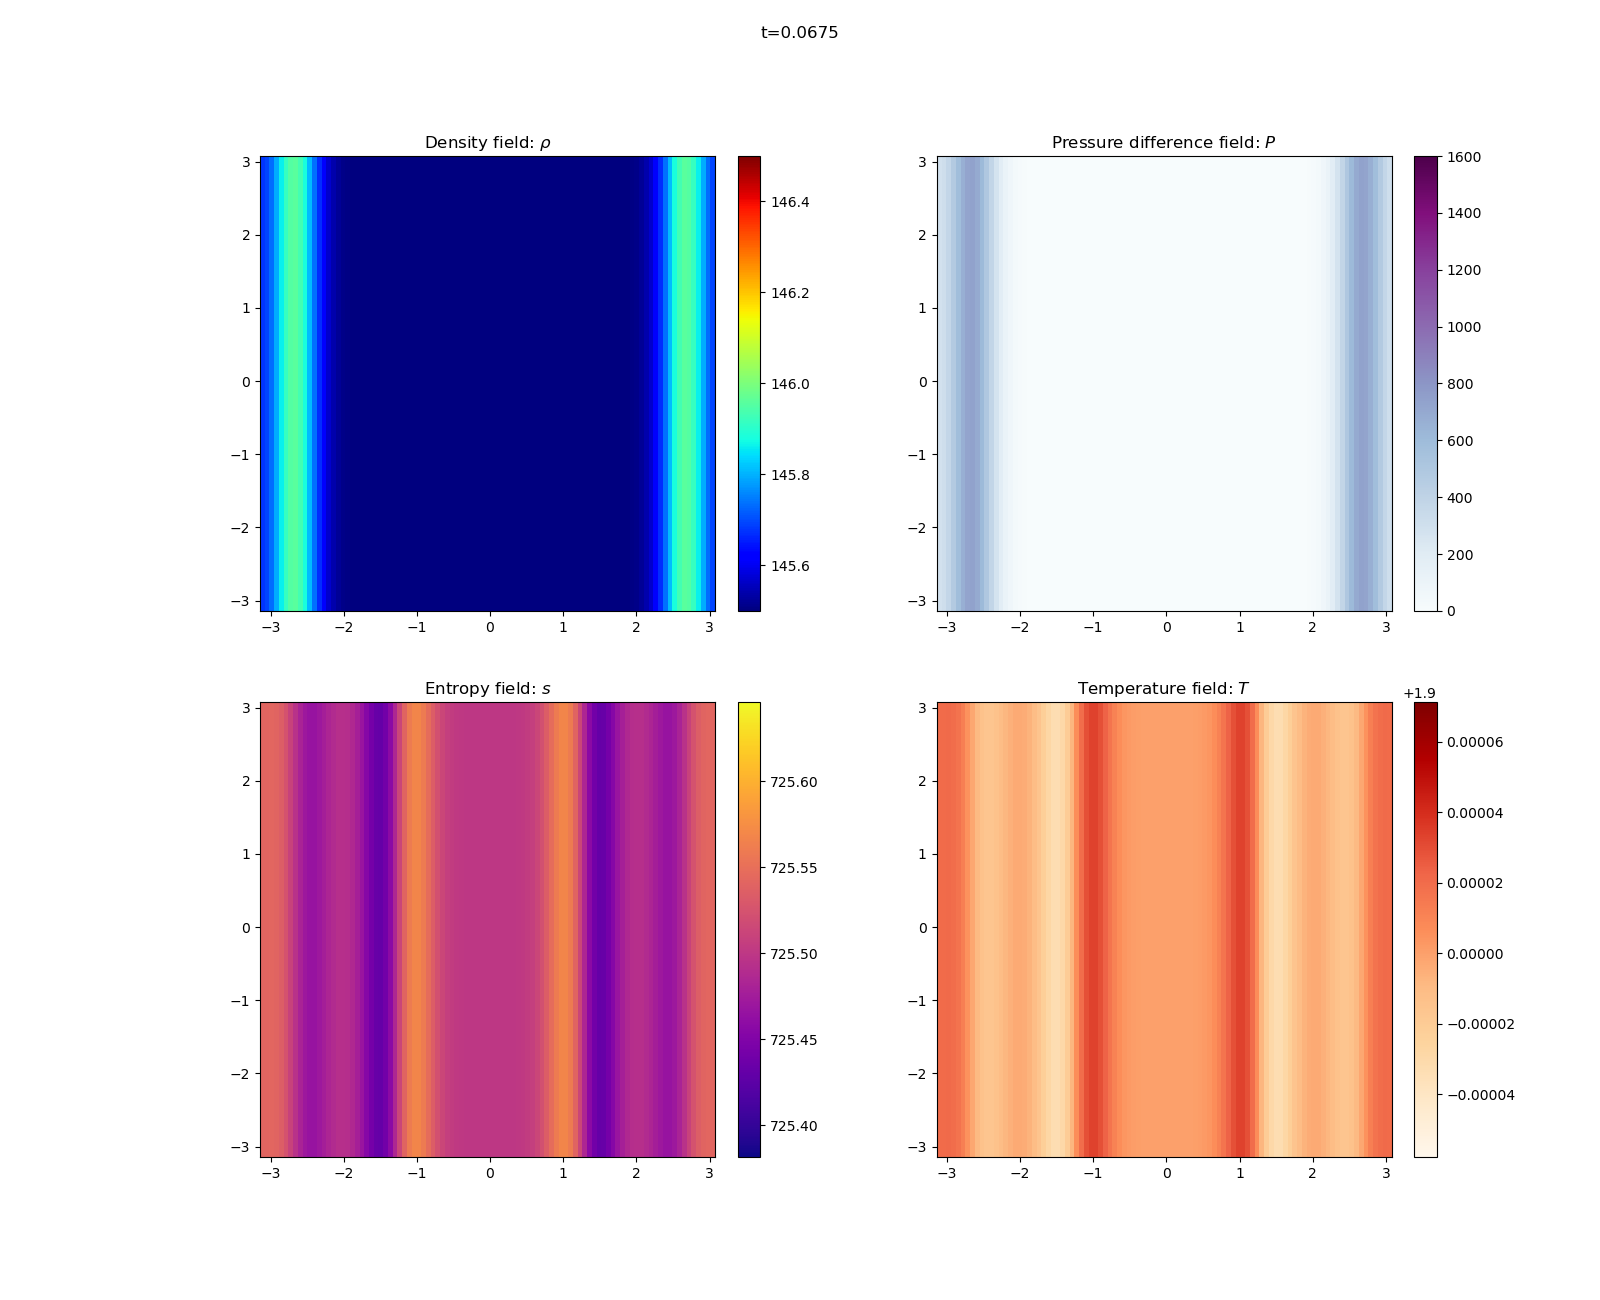
\includegraphics[width=\textwidth/3]{Sim 2/SF02_0027.png}
    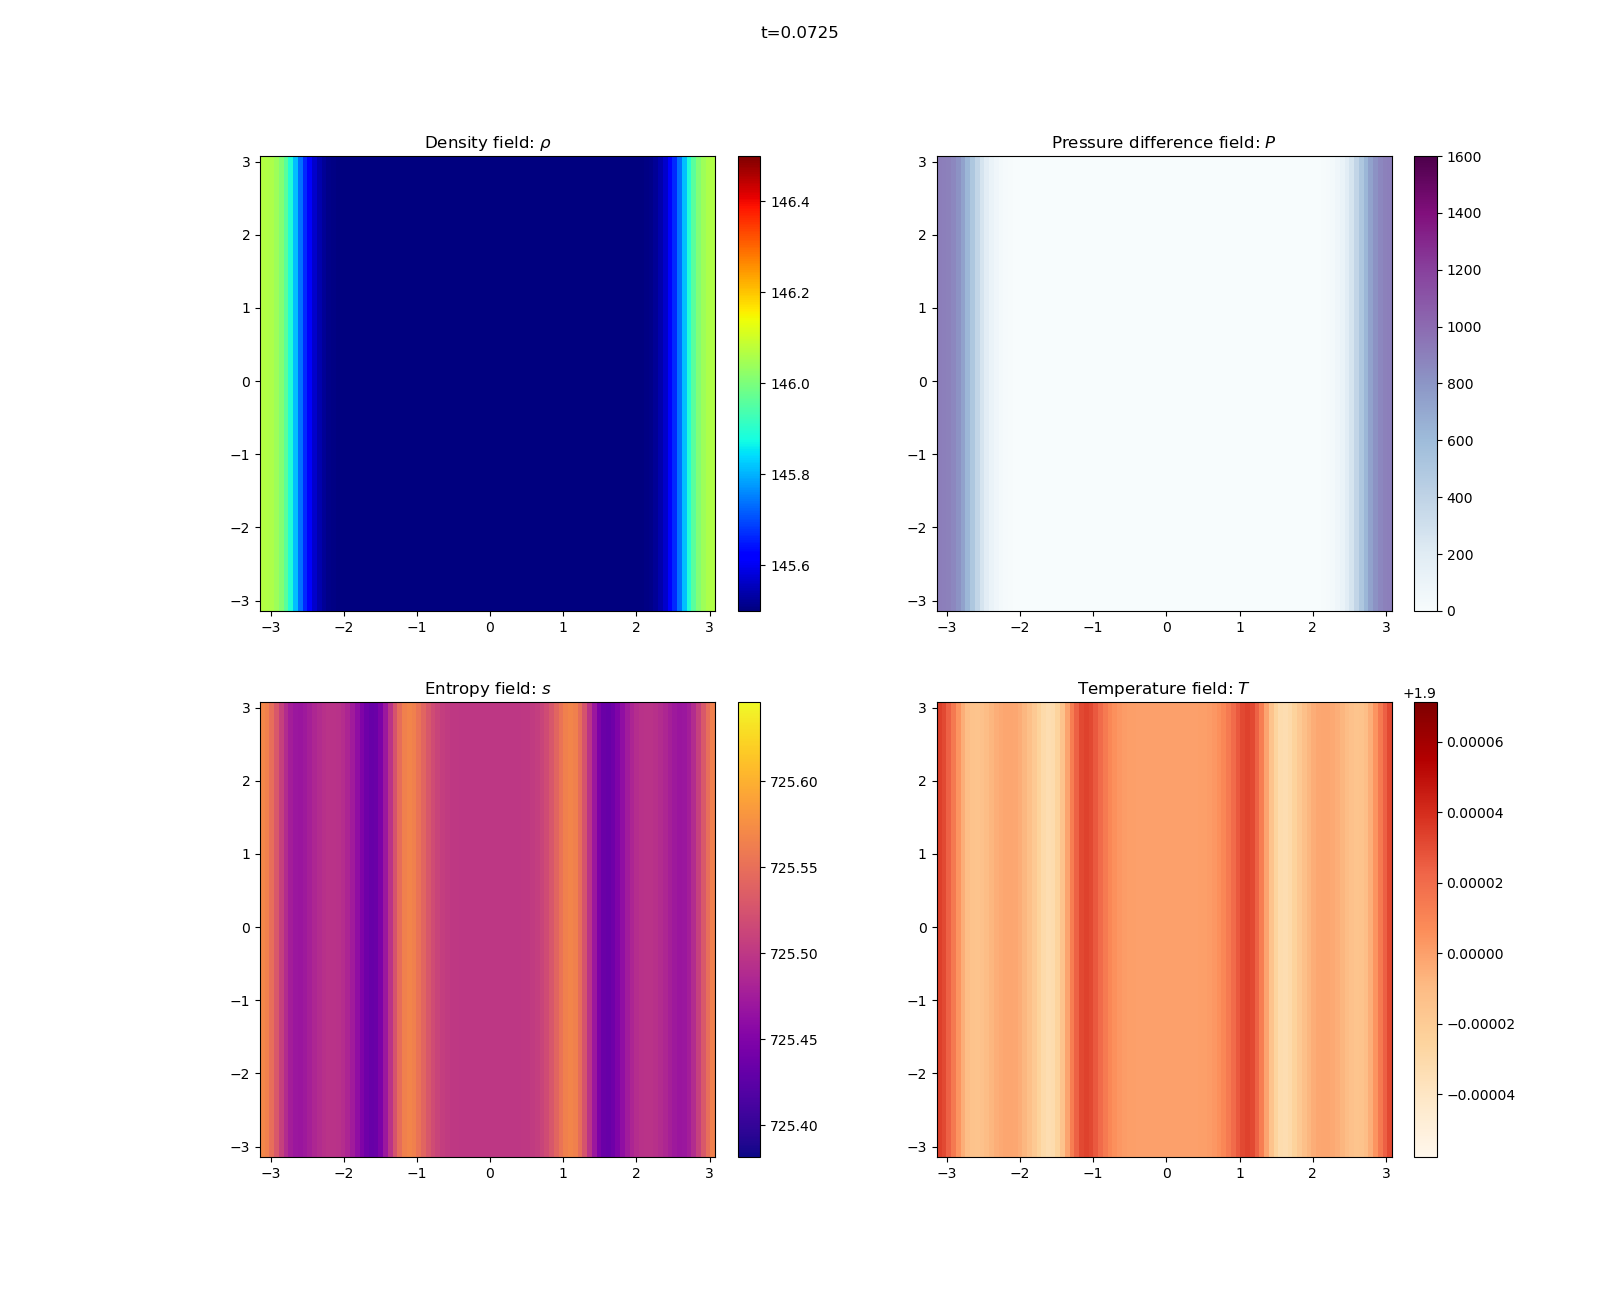
\includegraphics[width=\textwidth/3]{Sim 2/SF02_0029.png}
    \caption{Snapshots from simulation 3}
    \label{sim3}
\end{figure}

\section{Conclusion}

\todo{Write conclusion}
 
\section{Acknowledgements}

\todo{Ondřej Kincl}

\bibliographystyle{alpha} % Choose a style (e.g., plain, alpha, IEEEtran)
\bibliography{bibliography} % Point to your .bib file (without extension)

\todo{Bibliography}

\end{document}
